\documentclass[twoside]{book}

% Packages required by doxygen
\usepackage{calc}
\usepackage{doxygen}
\usepackage{graphicx}
\usepackage[utf8]{inputenc}
\usepackage{makeidx}
\usepackage{multicol}
\usepackage{multirow}
\usepackage{textcomp}
\usepackage[table]{xcolor}

% Font selection
\usepackage[T1]{fontenc}
\usepackage{mathptmx}
\usepackage[scaled=.90]{helvet}
\usepackage{courier}
\usepackage{amssymb}
\usepackage{sectsty}
\renewcommand{\familydefault}{\sfdefault}
\allsectionsfont{%
  \fontseries{bc}\selectfont%
  \color{darkgray}%
}
\renewcommand{\DoxyLabelFont}{%
  \fontseries{bc}\selectfont%
  \color{darkgray}%
}

% Page & text layout
\usepackage{geometry}
\geometry{%
  a4paper,%
  top=2.5cm,%
  bottom=2.5cm,%
  left=2.5cm,%
  right=2.5cm%
}
\tolerance=750
\hfuzz=15pt
\hbadness=750
\setlength{\emergencystretch}{15pt}
\setlength{\parindent}{0cm}
\setlength{\parskip}{0.2cm}
\makeatletter
\renewcommand{\paragraph}{%
  \@startsection{paragraph}{4}{0ex}{-1.0ex}{1.0ex}{%
    \normalfont\normalsize\bfseries\SS@parafont%
  }%
}
\renewcommand{\subparagraph}{%
  \@startsection{subparagraph}{5}{0ex}{-1.0ex}{1.0ex}{%
    \normalfont\normalsize\bfseries\SS@subparafont%
  }%
}
\makeatother

% Headers & footers
\usepackage{fancyhdr}
\pagestyle{fancyplain}
\fancyhead[LE]{\fancyplain{}{\bfseries\thepage}}
\fancyhead[CE]{\fancyplain{}{}}
\fancyhead[RE]{\fancyplain{}{\bfseries\leftmark}}
\fancyhead[LO]{\fancyplain{}{\bfseries\rightmark}}
\fancyhead[CO]{\fancyplain{}{}}
\fancyhead[RO]{\fancyplain{}{\bfseries\thepage}}
\fancyfoot[LE]{\fancyplain{}{}}
\fancyfoot[CE]{\fancyplain{}{}}
\fancyfoot[RE]{\fancyplain{}{\bfseries\scriptsize Generated on Wed Dec 11 2013 19\-:12\-:52 for Hamcrest-\/\-Qt by Doxygen }}
\fancyfoot[LO]{\fancyplain{}{\bfseries\scriptsize Generated on Wed Dec 11 2013 19\-:12\-:52 for Hamcrest-\/\-Qt by Doxygen }}
\fancyfoot[CO]{\fancyplain{}{}}
\fancyfoot[RO]{\fancyplain{}{}}
\renewcommand{\footrulewidth}{0.4pt}
\renewcommand{\chaptermark}[1]{%
  \markboth{#1}{}%
}
\renewcommand{\sectionmark}[1]{%
  \markright{\thesection\ #1}%
}

% Indices & bibliography
\usepackage{natbib}
\usepackage[titles]{tocloft}
\setcounter{tocdepth}{3}
\setcounter{secnumdepth}{5}
\makeindex

% Hyperlinks (required, but should be loaded last)
\usepackage{ifpdf}
\ifpdf
  \usepackage[pdftex,pagebackref=true]{hyperref}
\else
  \usepackage[ps2pdf,pagebackref=true]{hyperref}
\fi
\hypersetup{%
  colorlinks=true,%
  linkcolor=blue,%
  citecolor=blue,%
  unicode%
}

% Custom commands
\newcommand{\clearemptydoublepage}{%
  \newpage{\pagestyle{empty}\cleardoublepage}%
}


%===== C O N T E N T S =====

\begin{document}

% Titlepage & ToC
\hypersetup{pageanchor=false}
\pagenumbering{roman}
\begin{titlepage}
\vspace*{7cm}
\begin{center}%
{\Large Hamcrest-\/\-Qt \\[1ex]\large 0.\-0.\-1 }\\
\vspace*{1cm}
{\large Generated by Doxygen 1.8.5}\\
\vspace*{0.5cm}
{\small Wed Dec 11 2013 19:12:52}\\
\end{center}
\end{titlepage}
\clearemptydoublepage
\tableofcontents
\clearemptydoublepage
\pagenumbering{arabic}
\hypersetup{pageanchor=true}

%--- Begin generated contents ---
\chapter{Namespace Index}
\section{Namespace List}
Here is a list of all documented namespaces with brief descriptions\-:\begin{DoxyCompactList}
\item\contentsline{section}{\hyperlink{namespace_hamcrest_qt}{Hamcrest\-Qt} \\*Hamcrest-\/\-Qt is a library of matchers, which can be combined in to create flexible expressions of intent in tests }{\pageref{namespace_hamcrest_qt}}{}
\end{DoxyCompactList}

\chapter{Hierarchical Index}
\section{Class Hierarchy}
This inheritance list is sorted roughly, but not completely, alphabetically\-:\begin{DoxyCompactList}
\item \contentsline{section}{Hamcrest\-Qt\-:\-:Matcher\-Assert\-:\-:Assertion\-Listener}{\pageref{class_hamcrest_qt_1_1_matcher_assert_1_1_assertion_listener}}{}
\item \contentsline{section}{Hamcrest\-Qt\-:\-:Description}{\pageref{class_hamcrest_qt_1_1_description}}{}
\begin{DoxyCompactList}
\item \contentsline{section}{Hamcrest\-Qt\-:\-:Base\-Description}{\pageref{class_hamcrest_qt_1_1_base_description}}{}
\begin{DoxyCompactList}
\item \contentsline{section}{Hamcrest\-Qt\-:\-:String\-Description}{\pageref{class_hamcrest_qt_1_1_string_description}}{}
\end{DoxyCompactList}
\item \contentsline{section}{Hamcrest\-Qt\-:\-:Description\-:\-:Null\-Description}{\pageref{class_hamcrest_qt_1_1_description_1_1_null_description}}{}
\end{DoxyCompactList}
\item \contentsline{section}{Hamcrest\-Qt\-:\-:Matcher\-Assert}{\pageref{class_hamcrest_qt_1_1_matcher_assert}}{}
\item \contentsline{section}{Hamcrest\-Qt\-:\-:Self\-Describing}{\pageref{class_hamcrest_qt_1_1_self_describing}}{}
\begin{DoxyCompactList}
\item \contentsline{section}{Hamcrest\-Qt\-:\-:Matcher$<$ T $>$}{\pageref{class_hamcrest_qt_1_1_matcher}}{}
\begin{DoxyCompactList}
\item \contentsline{section}{Hamcrest\-Qt\-:\-:Base\-Matcher$<$ T $>$}{\pageref{class_hamcrest_qt_1_1_base_matcher}}{}
\begin{DoxyCompactList}
\item \contentsline{section}{Hamcrest\-Qt\-:\-:Diagnosing\-Matcher$<$ T $>$}{\pageref{class_hamcrest_qt_1_1_diagnosing_matcher}}{}
\begin{DoxyCompactList}
\item \contentsline{section}{Hamcrest\-Qt\-:\-:All\-Of$<$ T $>$}{\pageref{class_hamcrest_qt_1_1_all_of}}{}
\end{DoxyCompactList}
\item \contentsline{section}{Hamcrest\-Qt\-:\-:Is$<$ T $>$}{\pageref{class_hamcrest_qt_1_1_is}}{}
\item \contentsline{section}{Hamcrest\-Qt\-:\-:Is\-Equal$<$ T $>$}{\pageref{class_hamcrest_qt_1_1_is_equal}}{}
\item \contentsline{section}{Hamcrest\-Qt\-:\-:Is\-Not$<$ T $>$}{\pageref{class_hamcrest_qt_1_1_is_not}}{}
\item \contentsline{section}{Hamcrest\-Qt\-:\-:Shortcut\-Combination$<$ T $>$}{\pageref{class_hamcrest_qt_1_1_shortcut_combination}}{}
\begin{DoxyCompactList}
\item \contentsline{section}{Hamcrest\-Qt\-:\-:Any\-Of$<$ T $>$}{\pageref{class_hamcrest_qt_1_1_any_of}}{}
\end{DoxyCompactList}
\end{DoxyCompactList}
\end{DoxyCompactList}
\item \contentsline{section}{Hamcrest\-Qt\-:\-:Matcher$<$ Q\-String $>$}{\pageref{class_hamcrest_qt_1_1_matcher}}{}
\begin{DoxyCompactList}
\item \contentsline{section}{Hamcrest\-Qt\-:\-:Base\-Matcher$<$ Q\-String $>$}{\pageref{class_hamcrest_qt_1_1_base_matcher}}{}
\begin{DoxyCompactList}
\item \contentsline{section}{Hamcrest\-Qt\-:\-:Substring\-Matcher}{\pageref{class_hamcrest_qt_1_1_substring_matcher}}{}
\begin{DoxyCompactList}
\item \contentsline{section}{Hamcrest\-Qt\-:\-:String\-Contains}{\pageref{class_hamcrest_qt_1_1_string_contains}}{}
\item \contentsline{section}{Hamcrest\-Qt\-:\-:String\-Ends\-With}{\pageref{class_hamcrest_qt_1_1_string_ends_with}}{}
\item \contentsline{section}{Hamcrest\-Qt\-:\-:String\-Starts\-With}{\pageref{class_hamcrest_qt_1_1_string_starts_with}}{}
\end{DoxyCompactList}
\end{DoxyCompactList}
\end{DoxyCompactList}
\end{DoxyCompactList}
\end{DoxyCompactList}

\chapter{Class Index}
\section{Class List}
Here are the classes, structs, unions and interfaces with brief descriptions\-:\begin{DoxyCompactList}
\item\contentsline{section}{\hyperlink{class_hamcrest_qt_1_1_all_of}{Hamcrest\-Qt\-::\-All\-Of$<$ T $>$} \\*Calculates the logical conjunction of multiple matchers }{\pageref{class_hamcrest_qt_1_1_all_of}}{}
\item\contentsline{section}{\hyperlink{class_hamcrest_qt_1_1_any_of}{Hamcrest\-Qt\-::\-Any\-Of$<$ T $>$} \\*Calculates the logical disjunction of multiple matchers }{\pageref{class_hamcrest_qt_1_1_any_of}}{}
\item\contentsline{section}{\hyperlink{class_hamcrest_qt_1_1_matcher_assert_1_1_assertion_listener}{Hamcrest\-Qt\-::\-Matcher\-Assert\-::\-Assertion\-Listener} }{\pageref{class_hamcrest_qt_1_1_matcher_assert_1_1_assertion_listener}}{}
\item\contentsline{section}{\hyperlink{class_hamcrest_qt_1_1_base_description}{Hamcrest\-Qt\-::\-Base\-Description} \\*A \hyperlink{class_hamcrest_qt_1_1_description}{Description} that is stored as a string }{\pageref{class_hamcrest_qt_1_1_base_description}}{}
\item\contentsline{section}{\hyperlink{class_hamcrest_qt_1_1_base_matcher}{Hamcrest\-Qt\-::\-Base\-Matcher$<$ T $>$} \\*Base\-Class for all \hyperlink{class_hamcrest_qt_1_1_matcher}{Matcher} implementations }{\pageref{class_hamcrest_qt_1_1_base_matcher}}{}
\item\contentsline{section}{\hyperlink{class_hamcrest_qt_1_1_description}{Hamcrest\-Qt\-::\-Description} \\*A description of a \hyperlink{class_hamcrest_qt_1_1_matcher}{Matcher} }{\pageref{class_hamcrest_qt_1_1_description}}{}
\item\contentsline{section}{\hyperlink{class_hamcrest_qt_1_1_diagnosing_matcher}{Hamcrest\-Qt\-::\-Diagnosing\-Matcher$<$ T $>$} }{\pageref{class_hamcrest_qt_1_1_diagnosing_matcher}}{}
\item\contentsline{section}{\hyperlink{class_hamcrest_qt_1_1_is}{Hamcrest\-Qt\-::\-Is$<$ T $>$} \\*Decorates another \hyperlink{class_hamcrest_qt_1_1_matcher}{Matcher}, retaining the behaviour but allowing tests to be slightly more expressive }{\pageref{class_hamcrest_qt_1_1_is}}{}
\item\contentsline{section}{\hyperlink{class_hamcrest_qt_1_1_is_equal}{Hamcrest\-Qt\-::\-Is\-Equal$<$ T $>$} \\*\hyperlink{class_hamcrest_qt_1_1_is}{Is} the value equal to another value, as tested by the operator==() method? }{\pageref{class_hamcrest_qt_1_1_is_equal}}{}
\item\contentsline{section}{\hyperlink{class_hamcrest_qt_1_1_is_not}{Hamcrest\-Qt\-::\-Is\-Not$<$ T $>$} \\*Calculates the logical negation of a matcher }{\pageref{class_hamcrest_qt_1_1_is_not}}{}
\item\contentsline{section}{\hyperlink{class_hamcrest_qt_1_1_matcher}{Hamcrest\-Qt\-::\-Matcher$<$ T $>$} \\*A matcher over acceptable values }{\pageref{class_hamcrest_qt_1_1_matcher}}{}
\item\contentsline{section}{\hyperlink{class_hamcrest_qt_1_1_matcher_assert}{Hamcrest\-Qt\-::\-Matcher\-Assert} }{\pageref{class_hamcrest_qt_1_1_matcher_assert}}{}
\item\contentsline{section}{\hyperlink{class_hamcrest_qt_1_1_description_1_1_null_description}{Hamcrest\-Qt\-::\-Description\-::\-Null\-Description} }{\pageref{class_hamcrest_qt_1_1_description_1_1_null_description}}{}
\item\contentsline{section}{\hyperlink{class_hamcrest_qt_1_1_self_describing}{Hamcrest\-Qt\-::\-Self\-Describing} \\*The ability of an object to describe itself }{\pageref{class_hamcrest_qt_1_1_self_describing}}{}
\item\contentsline{section}{\hyperlink{class_hamcrest_qt_1_1_shortcut_combination}{Hamcrest\-Qt\-::\-Shortcut\-Combination$<$ T $>$} }{\pageref{class_hamcrest_qt_1_1_shortcut_combination}}{}
\item\contentsline{section}{\hyperlink{class_hamcrest_qt_1_1_string_contains}{Hamcrest\-Qt\-::\-String\-Contains} \\*Tests if the argument is a string that contains a substring }{\pageref{class_hamcrest_qt_1_1_string_contains}}{}
\item\contentsline{section}{\hyperlink{class_hamcrest_qt_1_1_string_description}{Hamcrest\-Qt\-::\-String\-Description} \\*A \hyperlink{class_hamcrest_qt_1_1_description}{Description} that is stored as a string }{\pageref{class_hamcrest_qt_1_1_string_description}}{}
\item\contentsline{section}{\hyperlink{class_hamcrest_qt_1_1_string_ends_with}{Hamcrest\-Qt\-::\-String\-Ends\-With} \\*Tests if the argument is a string that ends with a substring }{\pageref{class_hamcrest_qt_1_1_string_ends_with}}{}
\item\contentsline{section}{\hyperlink{class_hamcrest_qt_1_1_string_starts_with}{Hamcrest\-Qt\-::\-String\-Starts\-With} \\*Tests if the argument is a string that starts with a substring }{\pageref{class_hamcrest_qt_1_1_string_starts_with}}{}
\item\contentsline{section}{\hyperlink{class_hamcrest_qt_1_1_substring_matcher}{Hamcrest\-Qt\-::\-Substring\-Matcher} }{\pageref{class_hamcrest_qt_1_1_substring_matcher}}{}
\end{DoxyCompactList}

\chapter{Namespace Documentation}
\hypertarget{namespace_hamcrest_qt}{\section{Hamcrest\-Qt Namespace Reference}
\label{namespace_hamcrest_qt}\index{Hamcrest\-Qt@{Hamcrest\-Qt}}
}


Hamcrest-\/\-Qt is a library of matchers, which can be combined in to create flexible expressions of intent in tests.  


\subsection*{Classes}
\begin{DoxyCompactItemize}
\item 
class \hyperlink{class_hamcrest_qt_1_1_base_description}{Base\-Description}
\begin{DoxyCompactList}\small\item\em A \hyperlink{class_hamcrest_qt_1_1_description}{Description} that is stored as a string. \end{DoxyCompactList}\item 
class \hyperlink{class_hamcrest_qt_1_1_base_matcher}{Base\-Matcher}
\begin{DoxyCompactList}\small\item\em Base\-Class for all \hyperlink{class_hamcrest_qt_1_1_matcher}{Matcher} implementations. \end{DoxyCompactList}\item 
class \hyperlink{class_hamcrest_qt_1_1_description}{Description}
\begin{DoxyCompactList}\small\item\em A description of a \hyperlink{class_hamcrest_qt_1_1_matcher}{Matcher}. \end{DoxyCompactList}\item 
class \hyperlink{class_hamcrest_qt_1_1_diagnosing_matcher}{Diagnosing\-Matcher}
\item 
class \hyperlink{class_hamcrest_qt_1_1_all_of}{All\-Of}
\begin{DoxyCompactList}\small\item\em Calculates the logical conjunction of multiple matchers. \end{DoxyCompactList}\item 
class \hyperlink{class_hamcrest_qt_1_1_any_of}{Any\-Of}
\begin{DoxyCompactList}\small\item\em Calculates the logical disjunction of multiple matchers. \end{DoxyCompactList}\item 
class \hyperlink{class_hamcrest_qt_1_1_is}{Is}
\begin{DoxyCompactList}\small\item\em Decorates another \hyperlink{class_hamcrest_qt_1_1_matcher}{Matcher}, retaining the behaviour but allowing tests to be slightly more expressive. \end{DoxyCompactList}\item 
class \hyperlink{class_hamcrest_qt_1_1_is_equal}{Is\-Equal}
\begin{DoxyCompactList}\small\item\em \hyperlink{class_hamcrest_qt_1_1_is}{Is} the value equal to another value, as tested by the operator==() method? \end{DoxyCompactList}\item 
class \hyperlink{class_hamcrest_qt_1_1_is_not}{Is\-Not}
\begin{DoxyCompactList}\small\item\em Calculates the logical negation of a matcher. \end{DoxyCompactList}\item 
class \hyperlink{class_hamcrest_qt_1_1_shortcut_combination}{Shortcut\-Combination}
\item 
class \hyperlink{class_hamcrest_qt_1_1_string_contains}{String\-Contains}
\begin{DoxyCompactList}\small\item\em Tests if the argument is a string that contains a substring. \end{DoxyCompactList}\item 
class \hyperlink{class_hamcrest_qt_1_1_string_ends_with}{String\-Ends\-With}
\begin{DoxyCompactList}\small\item\em Tests if the argument is a string that ends with a substring. \end{DoxyCompactList}\item 
class \hyperlink{class_hamcrest_qt_1_1_string_starts_with}{String\-Starts\-With}
\begin{DoxyCompactList}\small\item\em Tests if the argument is a string that starts with a substring. \end{DoxyCompactList}\item 
class \hyperlink{class_hamcrest_qt_1_1_substring_matcher}{Substring\-Matcher}
\item 
class \hyperlink{class_hamcrest_qt_1_1_matcher}{Matcher}
\begin{DoxyCompactList}\small\item\em A matcher over acceptable values. \end{DoxyCompactList}\item 
class \hyperlink{class_hamcrest_qt_1_1_matcher_assert}{Matcher\-Assert}
\item 
class \hyperlink{class_hamcrest_qt_1_1_self_describing}{Self\-Describing}
\begin{DoxyCompactList}\small\item\em The ability of an object to describe itself. \end{DoxyCompactList}\item 
class \hyperlink{class_hamcrest_qt_1_1_string_description}{String\-Description}
\begin{DoxyCompactList}\small\item\em A \hyperlink{class_hamcrest_qt_1_1_description}{Description} that is stored as a string. \end{DoxyCompactList}\end{DoxyCompactItemize}
\subsection*{Functions}
\begin{DoxyCompactItemize}
\item 
{\footnotesize template$<$typename T $>$ }\\Q\-Shared\-Pointer$<$ \hyperlink{class_hamcrest_qt_1_1_matcher}{Matcher}$<$ T $>$ $>$ \hyperlink{namespace_hamcrest_qt_a77b3b27a3c856ef459926f4f8ec60307}{all\-Of} (const Q\-List$<$ Q\-Shared\-Pointer$<$ \hyperlink{class_hamcrest_qt_1_1_matcher}{Matcher}$<$ T $>$ $>$ $>$ \&matchers)
\begin{DoxyCompactList}\small\item\em Creates a matcher that matches if the examined object matches {\bfseries A\-L\-L} of the specified matchers. \end{DoxyCompactList}\item 
\hypertarget{namespace_hamcrest_qt_a9beec73c27114304f22a4704842bf841}{{\footnotesize template$<$typename T $>$ }\\Q\-Shared\-Pointer$<$ \hyperlink{class_hamcrest_qt_1_1_matcher}{Matcher}$<$ T $>$ $>$ {\bfseries all\-Of} (const Q\-Shared\-Pointer$<$ \hyperlink{class_hamcrest_qt_1_1_matcher}{Matcher}$<$ T $>$ $>$ \&first, const Q\-Shared\-Pointer$<$ \hyperlink{class_hamcrest_qt_1_1_matcher}{Matcher}$<$ T $>$ $>$ \&second)}\label{namespace_hamcrest_qt_a9beec73c27114304f22a4704842bf841}

\item 
\hypertarget{namespace_hamcrest_qt_a63a6d0c4bb869944c6bc4a6ce33a91cd}{{\footnotesize template$<$typename T $>$ }\\Q\-Shared\-Pointer$<$ \hyperlink{class_hamcrest_qt_1_1_matcher}{Matcher}$<$ T $>$ $>$ {\bfseries all\-Of} (const Q\-Shared\-Pointer$<$ \hyperlink{class_hamcrest_qt_1_1_matcher}{Matcher}$<$ T $>$ $>$ \&first, const Q\-Shared\-Pointer$<$ \hyperlink{class_hamcrest_qt_1_1_matcher}{Matcher}$<$ T $>$ $>$ \&second, const Q\-Shared\-Pointer$<$ \hyperlink{class_hamcrest_qt_1_1_matcher}{Matcher}$<$ T $>$ $>$ \&third)}\label{namespace_hamcrest_qt_a63a6d0c4bb869944c6bc4a6ce33a91cd}

\item 
\hypertarget{namespace_hamcrest_qt_af167d28bc118963c7b42598ce81a8fd5}{{\footnotesize template$<$typename T $>$ }\\Q\-Shared\-Pointer$<$ \hyperlink{class_hamcrest_qt_1_1_matcher}{Matcher}$<$ T $>$ $>$ {\bfseries all\-Of} (const Q\-Shared\-Pointer$<$ \hyperlink{class_hamcrest_qt_1_1_matcher}{Matcher}$<$ T $>$ $>$ \&first, const Q\-Shared\-Pointer$<$ \hyperlink{class_hamcrest_qt_1_1_matcher}{Matcher}$<$ T $>$ $>$ \&second, const Q\-Shared\-Pointer$<$ \hyperlink{class_hamcrest_qt_1_1_matcher}{Matcher}$<$ T $>$ $>$ \&third, const Q\-Shared\-Pointer$<$ \hyperlink{class_hamcrest_qt_1_1_matcher}{Matcher}$<$ T $>$ $>$ \&fourth)}\label{namespace_hamcrest_qt_af167d28bc118963c7b42598ce81a8fd5}

\item 
\hypertarget{namespace_hamcrest_qt_ade5face79ec28843e874d5838a6359a0}{{\footnotesize template$<$typename T $>$ }\\Q\-Shared\-Pointer$<$ \hyperlink{class_hamcrest_qt_1_1_matcher}{Matcher}$<$ T $>$ $>$ {\bfseries all\-Of} (const Q\-Shared\-Pointer$<$ \hyperlink{class_hamcrest_qt_1_1_matcher}{Matcher}$<$ T $>$ $>$ \&first, const Q\-Shared\-Pointer$<$ \hyperlink{class_hamcrest_qt_1_1_matcher}{Matcher}$<$ T $>$ $>$ \&second, const Q\-Shared\-Pointer$<$ \hyperlink{class_hamcrest_qt_1_1_matcher}{Matcher}$<$ T $>$ $>$ \&third, const Q\-Shared\-Pointer$<$ \hyperlink{class_hamcrest_qt_1_1_matcher}{Matcher}$<$ T $>$ $>$ \&fourth, const Q\-Shared\-Pointer$<$ \hyperlink{class_hamcrest_qt_1_1_matcher}{Matcher}$<$ T $>$ $>$ \&fifth)}\label{namespace_hamcrest_qt_ade5face79ec28843e874d5838a6359a0}

\item 
\hypertarget{namespace_hamcrest_qt_a212acd440c9c1c5cfc353746658ef4ae}{{\footnotesize template$<$typename T $>$ }\\Q\-Shared\-Pointer$<$ \hyperlink{class_hamcrest_qt_1_1_matcher}{Matcher}$<$ T $>$ $>$ {\bfseries all\-Of} (const Q\-Shared\-Pointer$<$ \hyperlink{class_hamcrest_qt_1_1_matcher}{Matcher}$<$ T $>$ $>$ \&first, const Q\-Shared\-Pointer$<$ \hyperlink{class_hamcrest_qt_1_1_matcher}{Matcher}$<$ T $>$ $>$ \&second, const Q\-Shared\-Pointer$<$ \hyperlink{class_hamcrest_qt_1_1_matcher}{Matcher}$<$ T $>$ $>$ \&third, const Q\-Shared\-Pointer$<$ \hyperlink{class_hamcrest_qt_1_1_matcher}{Matcher}$<$ T $>$ $>$ \&fourth, const Q\-Shared\-Pointer$<$ \hyperlink{class_hamcrest_qt_1_1_matcher}{Matcher}$<$ T $>$ $>$ \&fifth, const Q\-Shared\-Pointer$<$ \hyperlink{class_hamcrest_qt_1_1_matcher}{Matcher}$<$ T $>$ $>$ \&sixth)}\label{namespace_hamcrest_qt_a212acd440c9c1c5cfc353746658ef4ae}

\item 
{\footnotesize template$<$typename T $>$ }\\Q\-Shared\-Pointer$<$ \hyperlink{class_hamcrest_qt_1_1_matcher}{Matcher}$<$ T $>$ $>$ \hyperlink{namespace_hamcrest_qt_a3bdc7acaf499318972b745c8a21b0fb6}{any\-Of} (const Q\-List$<$ Q\-Shared\-Pointer$<$ \hyperlink{class_hamcrest_qt_1_1_matcher}{Matcher}$<$ T $>$ $>$ $>$ \&matchers)
\begin{DoxyCompactList}\small\item\em Creates a matcher that matches if the examined object matches {\bfseries A\-N\-Y} of the specified matchers. \end{DoxyCompactList}\item 
\hypertarget{namespace_hamcrest_qt_a87fd234ca8afe8ef6881c7df105ee989}{{\footnotesize template$<$typename T $>$ }\\Q\-Shared\-Pointer$<$ \hyperlink{class_hamcrest_qt_1_1_matcher}{Matcher}$<$ T $>$ $>$ {\bfseries any\-Of} (const Q\-Shared\-Pointer$<$ \hyperlink{class_hamcrest_qt_1_1_matcher}{Matcher}$<$ T $>$ $>$ \&first, const Q\-Shared\-Pointer$<$ \hyperlink{class_hamcrest_qt_1_1_matcher}{Matcher}$<$ T $>$ $>$ \&second)}\label{namespace_hamcrest_qt_a87fd234ca8afe8ef6881c7df105ee989}

\item 
\hypertarget{namespace_hamcrest_qt_a1849e87c7501720cdda6f61640eb99c2}{{\footnotesize template$<$typename T $>$ }\\Q\-Shared\-Pointer$<$ \hyperlink{class_hamcrest_qt_1_1_matcher}{Matcher}$<$ T $>$ $>$ {\bfseries any\-Of} (const Q\-Shared\-Pointer$<$ \hyperlink{class_hamcrest_qt_1_1_matcher}{Matcher}$<$ T $>$ $>$ \&first, const Q\-Shared\-Pointer$<$ \hyperlink{class_hamcrest_qt_1_1_matcher}{Matcher}$<$ T $>$ $>$ \&second, const Q\-Shared\-Pointer$<$ \hyperlink{class_hamcrest_qt_1_1_matcher}{Matcher}$<$ T $>$ $>$ \&third)}\label{namespace_hamcrest_qt_a1849e87c7501720cdda6f61640eb99c2}

\item 
\hypertarget{namespace_hamcrest_qt_a8e62bf0eb93327418df0aae733e36f73}{{\footnotesize template$<$typename T $>$ }\\Q\-Shared\-Pointer$<$ \hyperlink{class_hamcrest_qt_1_1_matcher}{Matcher}$<$ T $>$ $>$ {\bfseries any\-Of} (const Q\-Shared\-Pointer$<$ \hyperlink{class_hamcrest_qt_1_1_matcher}{Matcher}$<$ T $>$ $>$ \&first, const Q\-Shared\-Pointer$<$ \hyperlink{class_hamcrest_qt_1_1_matcher}{Matcher}$<$ T $>$ $>$ \&second, const Q\-Shared\-Pointer$<$ \hyperlink{class_hamcrest_qt_1_1_matcher}{Matcher}$<$ T $>$ $>$ \&third, const Q\-Shared\-Pointer$<$ \hyperlink{class_hamcrest_qt_1_1_matcher}{Matcher}$<$ T $>$ $>$ \&fourth)}\label{namespace_hamcrest_qt_a8e62bf0eb93327418df0aae733e36f73}

\item 
\hypertarget{namespace_hamcrest_qt_a55adc1b8685bb4cac50aa602d03c200d}{{\footnotesize template$<$typename T $>$ }\\Q\-Shared\-Pointer$<$ \hyperlink{class_hamcrest_qt_1_1_matcher}{Matcher}$<$ T $>$ $>$ {\bfseries any\-Of} (const Q\-Shared\-Pointer$<$ \hyperlink{class_hamcrest_qt_1_1_matcher}{Matcher}$<$ T $>$ $>$ \&first, const Q\-Shared\-Pointer$<$ \hyperlink{class_hamcrest_qt_1_1_matcher}{Matcher}$<$ T $>$ $>$ \&second, const Q\-Shared\-Pointer$<$ \hyperlink{class_hamcrest_qt_1_1_matcher}{Matcher}$<$ T $>$ $>$ \&third, const Q\-Shared\-Pointer$<$ \hyperlink{class_hamcrest_qt_1_1_matcher}{Matcher}$<$ T $>$ $>$ \&fourth, const Q\-Shared\-Pointer$<$ \hyperlink{class_hamcrest_qt_1_1_matcher}{Matcher}$<$ T $>$ $>$ \&fifth)}\label{namespace_hamcrest_qt_a55adc1b8685bb4cac50aa602d03c200d}

\item 
\hypertarget{namespace_hamcrest_qt_ab08811fbd4164f6ca3b700b48f528e1e}{{\footnotesize template$<$typename T $>$ }\\Q\-Shared\-Pointer$<$ \hyperlink{class_hamcrest_qt_1_1_matcher}{Matcher}$<$ T $>$ $>$ {\bfseries any\-Of} (const Q\-Shared\-Pointer$<$ \hyperlink{class_hamcrest_qt_1_1_matcher}{Matcher}$<$ T $>$ $>$ \&first, const Q\-Shared\-Pointer$<$ \hyperlink{class_hamcrest_qt_1_1_matcher}{Matcher}$<$ T $>$ $>$ \&second, const Q\-Shared\-Pointer$<$ \hyperlink{class_hamcrest_qt_1_1_matcher}{Matcher}$<$ T $>$ $>$ \&third, const Q\-Shared\-Pointer$<$ \hyperlink{class_hamcrest_qt_1_1_matcher}{Matcher}$<$ T $>$ $>$ \&fourth, const Q\-Shared\-Pointer$<$ \hyperlink{class_hamcrest_qt_1_1_matcher}{Matcher}$<$ T $>$ $>$ \&fifth, const Q\-Shared\-Pointer$<$ \hyperlink{class_hamcrest_qt_1_1_matcher}{Matcher}$<$ T $>$ $>$ \&sixth)}\label{namespace_hamcrest_qt_ab08811fbd4164f6ca3b700b48f528e1e}

\item 
\hypertarget{namespace_hamcrest_qt_a1a99fe898b2b85cb0a249123a44b3b6f}{{\footnotesize template$<$typename T $>$ }\\bool {\bfseries Are\-Equal} (const T \&actual, const T \&expected)}\label{namespace_hamcrest_qt_a1a99fe898b2b85cb0a249123a44b3b6f}

\item 
\hypertarget{namespace_hamcrest_qt_ae0acf05b2fd0a342d222bd30f9d82799}{bool {\bfseries Are\-Equal} (const char $\ast$actual, const char $\ast$expected)}\label{namespace_hamcrest_qt_ae0acf05b2fd0a342d222bd30f9d82799}

\item 
{\footnotesize template$<$typename T $>$ }\\Q\-Shared\-Pointer$<$ \hyperlink{class_hamcrest_qt_1_1_matcher}{Matcher}$<$ T $>$ $>$ \hyperlink{namespace_hamcrest_qt_af2c85daf497047f4891285dd0a86f7f1}{is} (const Q\-Shared\-Pointer$<$ \hyperlink{class_hamcrest_qt_1_1_matcher}{Matcher}$<$ T $>$ $>$ \&matcher)
\begin{DoxyCompactList}\small\item\em Decorates another \hyperlink{class_hamcrest_qt_1_1_matcher}{Matcher}, retaining its behaviour, but allowing tests to be slightly more expressive. \end{DoxyCompactList}\item 
\hypertarget{namespace_hamcrest_qt_a45dcba83f740365cbd95c2ea06ac2a3f}{{\footnotesize template$<$typename T $>$ }\\Q\-Shared\-Pointer$<$ \hyperlink{class_hamcrest_qt_1_1_matcher}{Matcher}$<$ T $>$ $>$ {\bfseries is} (const T \&operand)}\label{namespace_hamcrest_qt_a45dcba83f740365cbd95c2ea06ac2a3f}

\item 
\hypertarget{namespace_hamcrest_qt_aeee2510fdb711c6f7185b68e269ff2a9}{Q\-Shared\-Pointer$<$ \hyperlink{class_hamcrest_qt_1_1_matcher}{Matcher}$<$ const \\*
char $\ast$ $>$ $>$ {\bfseries is} (const char $\ast$operand)}\label{namespace_hamcrest_qt_aeee2510fdb711c6f7185b68e269ff2a9}

\item 
\hypertarget{namespace_hamcrest_qt_a117dd95db4e9739b9131ba7e3fa943c3}{{\footnotesize template$<$typename T $>$ }\\Q\-Shared\-Pointer$<$ \hyperlink{class_hamcrest_qt_1_1_matcher}{Matcher}$<$ T $>$ $>$ {\bfseries equal\-To} (const T \&operand)}\label{namespace_hamcrest_qt_a117dd95db4e9739b9131ba7e3fa943c3}

\item 
\hypertarget{namespace_hamcrest_qt_a69fe6ca6e07236c8071b760c8e1508a3}{Q\-Shared\-Pointer$<$ \hyperlink{class_hamcrest_qt_1_1_matcher}{Matcher}$<$ const \\*
char $\ast$ $>$ $>$ {\bfseries equal\-To} (const char operand\mbox{[}$\,$\mbox{]})}\label{namespace_hamcrest_qt_a69fe6ca6e07236c8071b760c8e1508a3}

\item 
{\footnotesize template$<$typename T $>$ }\\Q\-Shared\-Pointer$<$ \hyperlink{class_hamcrest_qt_1_1_matcher}{Matcher}$<$ T $>$ $>$ \hyperlink{namespace_hamcrest_qt_a1adc24012e56d9cd44b402873a3ffc03}{\-\_\-not} (const Q\-Shared\-Pointer$<$ \hyperlink{class_hamcrest_qt_1_1_matcher}{Matcher}$<$ T $>$ $>$ \&matcher)
\begin{DoxyCompactList}\small\item\em Creates a matcher that wraps an existing matcher, but inverts the logic by which it will match. \end{DoxyCompactList}\item 
{\footnotesize template$<$typename T $>$ }\\Q\-Shared\-Pointer$<$ \hyperlink{class_hamcrest_qt_1_1_matcher}{Matcher}$<$ T $>$ $>$ \hyperlink{namespace_hamcrest_qt_abfd16a389cc4dbec5004ba9c9d059660}{\-\_\-not} (const T \&operand)
\begin{DoxyCompactList}\small\item\em A shortcut to the frequently used {\ttfamily not(equal\-To(x))}. \end{DoxyCompactList}\item 
\hypertarget{namespace_hamcrest_qt_ae671e6aecabf951d073f2e0e4c0fb2b8}{Q\-Shared\-Pointer$<$ \hyperlink{class_hamcrest_qt_1_1_matcher}{Matcher}$<$ const \\*
char $\ast$ $>$ $>$ {\bfseries \-\_\-not} (const char $\ast$operand)}\label{namespace_hamcrest_qt_ae671e6aecabf951d073f2e0e4c0fb2b8}

\item 
Q\-Shared\-Pointer$<$ \hyperlink{class_hamcrest_qt_1_1_matcher}{Matcher}\\*
$<$ Q\-String $>$ $>$ \hyperlink{namespace_hamcrest_qt_ab456663a918a874b9fbf4c42dde6a439}{contains\-String} (const Q\-String \&substring)
\begin{DoxyCompactList}\small\item\em Creates a matcher that matches if the examined {\ttfamily Q\-String} contains the specified {\ttfamily Q\-String} anywhere. \end{DoxyCompactList}\item 
\hypertarget{namespace_hamcrest_qt_a4c961b244474f08f32c3c6523241c158}{Q\-Shared\-Pointer$<$ \hyperlink{class_hamcrest_qt_1_1_matcher}{Matcher}\\*
$<$ Q\-String $>$ $>$ {\bfseries contains\-String} (const char $\ast$substring)}\label{namespace_hamcrest_qt_a4c961b244474f08f32c3c6523241c158}

\item 
Q\-Shared\-Pointer$<$ \hyperlink{class_hamcrest_qt_1_1_matcher}{Matcher}\\*
$<$ Q\-String $>$ $>$ \hyperlink{namespace_hamcrest_qt_ae6827e66bbc17e98ac7bfc8bc256a399}{ends\-With} (const Q\-String \&suffix)
\begin{DoxyCompactList}\small\item\em Creates a matcher that matches if the examined {\ttfamily Q\-String} ends with the specified {\ttfamily Q\-String}. \end{DoxyCompactList}\item 
\hypertarget{namespace_hamcrest_qt_a43903b6fc354f9d0ff065192278bb62e}{Q\-Shared\-Pointer$<$ \hyperlink{class_hamcrest_qt_1_1_matcher}{Matcher}\\*
$<$ Q\-String $>$ $>$ {\bfseries ends\-With} (const char $\ast$suffix)}\label{namespace_hamcrest_qt_a43903b6fc354f9d0ff065192278bb62e}

\item 
Q\-Shared\-Pointer$<$ \hyperlink{class_hamcrest_qt_1_1_matcher}{Matcher}\\*
$<$ Q\-String $>$ $>$ \hyperlink{namespace_hamcrest_qt_a64e4b2a75d225fcd62ada49698f8614a}{starts\-With} (const Q\-String \&prefix)
\begin{DoxyCompactList}\small\item\em Creates a matcher that matches if the examined {\ttfamily Q\-String} starts with the specified {\ttfamily Q\-String}. \end{DoxyCompactList}\item 
\hypertarget{namespace_hamcrest_qt_a8631f62f98d1de7d44558107f0daf1f6}{Q\-Shared\-Pointer$<$ \hyperlink{class_hamcrest_qt_1_1_matcher}{Matcher}\\*
$<$ Q\-String $>$ $>$ {\bfseries starts\-With} (const char $\ast$prefix)}\label{namespace_hamcrest_qt_a8631f62f98d1de7d44558107f0daf1f6}

\end{DoxyCompactItemize}


\subsection{Detailed Description}
Hamcrest-\/\-Qt is a library of matchers, which can be combined in to create flexible expressions of intent in tests. 

\subsection{Function Documentation}
\hypertarget{namespace_hamcrest_qt_a1adc24012e56d9cd44b402873a3ffc03}{\index{Hamcrest\-Qt@{Hamcrest\-Qt}!\-\_\-not@{\-\_\-not}}
\index{\-\_\-not@{\-\_\-not}!HamcrestQt@{Hamcrest\-Qt}}
\subsubsection[{\-\_\-not}]{\setlength{\rightskip}{0pt plus 5cm}template$<$typename T $>$ Q\-Shared\-Pointer$<${\bf Matcher}$<$T$>$ $>$ Hamcrest\-Qt\-::\-\_\-not (
\begin{DoxyParamCaption}
\item[{const Q\-Shared\-Pointer$<$ Matcher$<$ T $>$ $>$ \&}]{matcher}
\end{DoxyParamCaption}
)}}\label{namespace_hamcrest_qt_a1adc24012e56d9cd44b402873a3ffc03}


Creates a matcher that wraps an existing matcher, but inverts the logic by which it will match. 

For example\-: 
\begin{DoxyPre}assertThat(cheese, is(not(equalTo(smelly))))\end{DoxyPre}



\begin{DoxyParams}{Parameters}
{\em matcher} & the matcher whose sense should be inverted \\
\hline
\end{DoxyParams}
\hypertarget{namespace_hamcrest_qt_abfd16a389cc4dbec5004ba9c9d059660}{\index{Hamcrest\-Qt@{Hamcrest\-Qt}!\-\_\-not@{\-\_\-not}}
\index{\-\_\-not@{\-\_\-not}!HamcrestQt@{Hamcrest\-Qt}}
\subsubsection[{\-\_\-not}]{\setlength{\rightskip}{0pt plus 5cm}template$<$typename T $>$ Q\-Shared\-Pointer$<${\bf Matcher}$<$T$>$ $>$ Hamcrest\-Qt\-::\-\_\-not (
\begin{DoxyParamCaption}
\item[{const T \&}]{operand}
\end{DoxyParamCaption}
)}}\label{namespace_hamcrest_qt_abfd16a389cc4dbec5004ba9c9d059660}


A shortcut to the frequently used {\ttfamily not(equal\-To(x))}. 

For example\-: 
\begin{DoxyPre}assertThat(cheese, is(not(smelly)))\end{DoxyPre}
 instead of\-: 
\begin{DoxyPre}assertThat(cheese, is(not(equalTo(smelly))))\end{DoxyPre}



\begin{DoxyParams}{Parameters}
{\em value} & the value that any examined object should {\bfseries not} equal \\
\hline
\end{DoxyParams}
\hypertarget{namespace_hamcrest_qt_a77b3b27a3c856ef459926f4f8ec60307}{\index{Hamcrest\-Qt@{Hamcrest\-Qt}!all\-Of@{all\-Of}}
\index{all\-Of@{all\-Of}!HamcrestQt@{Hamcrest\-Qt}}
\subsubsection[{all\-Of}]{\setlength{\rightskip}{0pt plus 5cm}template$<$typename T $>$ Q\-Shared\-Pointer$<${\bf Matcher}$<$T$>$ $>$ Hamcrest\-Qt\-::all\-Of (
\begin{DoxyParamCaption}
\item[{const Q\-List$<$ Q\-Shared\-Pointer$<$ Matcher$<$ T $>$ $>$ $>$ \&}]{matchers}
\end{DoxyParamCaption}
)}}\label{namespace_hamcrest_qt_a77b3b27a3c856ef459926f4f8ec60307}


Creates a matcher that matches if the examined object matches {\bfseries A\-L\-L} of the specified matchers. 

For example\-: 
\begin{DoxyPre}assertThat("myValue", allOf(startsWith("my"), containsString("Val")))\end{DoxyPre}
 \hypertarget{namespace_hamcrest_qt_a3bdc7acaf499318972b745c8a21b0fb6}{\index{Hamcrest\-Qt@{Hamcrest\-Qt}!any\-Of@{any\-Of}}
\index{any\-Of@{any\-Of}!HamcrestQt@{Hamcrest\-Qt}}
\subsubsection[{any\-Of}]{\setlength{\rightskip}{0pt plus 5cm}template$<$typename T $>$ Q\-Shared\-Pointer$<${\bf Matcher}$<$T$>$ $>$ Hamcrest\-Qt\-::any\-Of (
\begin{DoxyParamCaption}
\item[{const Q\-List$<$ Q\-Shared\-Pointer$<$ Matcher$<$ T $>$ $>$ $>$ \&}]{matchers}
\end{DoxyParamCaption}
)}}\label{namespace_hamcrest_qt_a3bdc7acaf499318972b745c8a21b0fb6}


Creates a matcher that matches if the examined object matches {\bfseries A\-N\-Y} of the specified matchers. 

For example\-: 
\begin{DoxyPre}assertThat("myValue", anyOf(startsWith("foo"), containsString("Val")))\end{DoxyPre}
 \hypertarget{namespace_hamcrest_qt_ab456663a918a874b9fbf4c42dde6a439}{\index{Hamcrest\-Qt@{Hamcrest\-Qt}!contains\-String@{contains\-String}}
\index{contains\-String@{contains\-String}!HamcrestQt@{Hamcrest\-Qt}}
\subsubsection[{contains\-String}]{\setlength{\rightskip}{0pt plus 5cm}Q\-Shared\-Pointer$<${\bf Matcher}$<$Q\-String$>$ $>$ Hamcrest\-Qt\-::contains\-String (
\begin{DoxyParamCaption}
\item[{const Q\-String \&}]{substring}
\end{DoxyParamCaption}
)\hspace{0.3cm}{\ttfamily [inline]}}}\label{namespace_hamcrest_qt_ab456663a918a874b9fbf4c42dde6a439}


Creates a matcher that matches if the examined {\ttfamily Q\-String} contains the specified {\ttfamily Q\-String} anywhere. 

For example\-: 
\begin{DoxyCode}
ASSERT\_THAT(\textcolor{stringliteral}{"myStringOfNote"}, \hyperlink{namespace_hamcrest_qt_ab456663a918a874b9fbf4c42dde6a439}{containsString}(\textcolor{stringliteral}{"ring"})); 
\end{DoxyCode}



\begin{DoxyParams}{Parameters}
{\em substring} & the substring that the returned matcher will expect to find within any examined string \\
\hline
\end{DoxyParams}
\hypertarget{namespace_hamcrest_qt_ae6827e66bbc17e98ac7bfc8bc256a399}{\index{Hamcrest\-Qt@{Hamcrest\-Qt}!ends\-With@{ends\-With}}
\index{ends\-With@{ends\-With}!HamcrestQt@{Hamcrest\-Qt}}
\subsubsection[{ends\-With}]{\setlength{\rightskip}{0pt plus 5cm}Q\-Shared\-Pointer$<${\bf Matcher}$<$Q\-String$>$ $>$ Hamcrest\-Qt\-::ends\-With (
\begin{DoxyParamCaption}
\item[{const Q\-String \&}]{suffix}
\end{DoxyParamCaption}
)\hspace{0.3cm}{\ttfamily [inline]}}}\label{namespace_hamcrest_qt_ae6827e66bbc17e98ac7bfc8bc256a399}


Creates a matcher that matches if the examined {\ttfamily Q\-String} ends with the specified {\ttfamily Q\-String}. 

For example\-: 
\begin{DoxyPre}assertThat("myStringOfNote", endsWith("Note"))\end{DoxyPre}



\begin{DoxyParams}{Parameters}
{\em suffix} & the substring that the returned matcher will expect at the end of any examined string \\
\hline
\end{DoxyParams}
\hypertarget{namespace_hamcrest_qt_af2c85daf497047f4891285dd0a86f7f1}{\index{Hamcrest\-Qt@{Hamcrest\-Qt}!is@{is}}
\index{is@{is}!HamcrestQt@{Hamcrest\-Qt}}
\subsubsection[{is}]{\setlength{\rightskip}{0pt plus 5cm}template$<$typename T $>$ Q\-Shared\-Pointer$<${\bf Matcher}$<$T$>$ $>$ Hamcrest\-Qt\-::is (
\begin{DoxyParamCaption}
\item[{const Q\-Shared\-Pointer$<$ Matcher$<$ T $>$ $>$ \&}]{matcher}
\end{DoxyParamCaption}
)}}\label{namespace_hamcrest_qt_af2c85daf497047f4891285dd0a86f7f1}


Decorates another \hyperlink{class_hamcrest_qt_1_1_matcher}{Matcher}, retaining its behaviour, but allowing tests to be slightly more expressive. 

For example\-: 
\begin{DoxyPre}assertThat(cheese, is(equalTo(smelly)))\end{DoxyPre}
 instead of\-: 
\begin{DoxyPre}assertThat(cheese, equalTo(smelly))\end{DoxyPre}
 \hypertarget{namespace_hamcrest_qt_a64e4b2a75d225fcd62ada49698f8614a}{\index{Hamcrest\-Qt@{Hamcrest\-Qt}!starts\-With@{starts\-With}}
\index{starts\-With@{starts\-With}!HamcrestQt@{Hamcrest\-Qt}}
\subsubsection[{starts\-With}]{\setlength{\rightskip}{0pt plus 5cm}Q\-Shared\-Pointer$<${\bf Matcher}$<$Q\-String$>$ $>$ Hamcrest\-Qt\-::starts\-With (
\begin{DoxyParamCaption}
\item[{const Q\-String \&}]{prefix}
\end{DoxyParamCaption}
)\hspace{0.3cm}{\ttfamily [inline]}}}\label{namespace_hamcrest_qt_a64e4b2a75d225fcd62ada49698f8614a}


Creates a matcher that matches if the examined {\ttfamily Q\-String} starts with the specified {\ttfamily Q\-String}. 

For example\-: 
\begin{DoxyPre}assertThat("myStringOfNote", startsWith("my"))\end{DoxyPre}



\begin{DoxyParams}{Parameters}
{\em prefix} & the substring that the returned matcher will expect at the start of any examined string \\
\hline
\end{DoxyParams}

\chapter{Class Documentation}
\hypertarget{class_hamcrest_qt_1_1_all_of}{\section{Hamcrest\-Qt\-:\-:All\-Of$<$ T $>$ Class Template Reference}
\label{class_hamcrest_qt_1_1_all_of}\index{Hamcrest\-Qt\-::\-All\-Of$<$ T $>$@{Hamcrest\-Qt\-::\-All\-Of$<$ T $>$}}
}


Calculates the logical conjunction of multiple matchers.  




{\ttfamily \#include $<$allof.\-h$>$}

Inheritance diagram for Hamcrest\-Qt\-:\-:All\-Of$<$ T $>$\-:\begin{figure}[H]
\begin{center}
\leavevmode
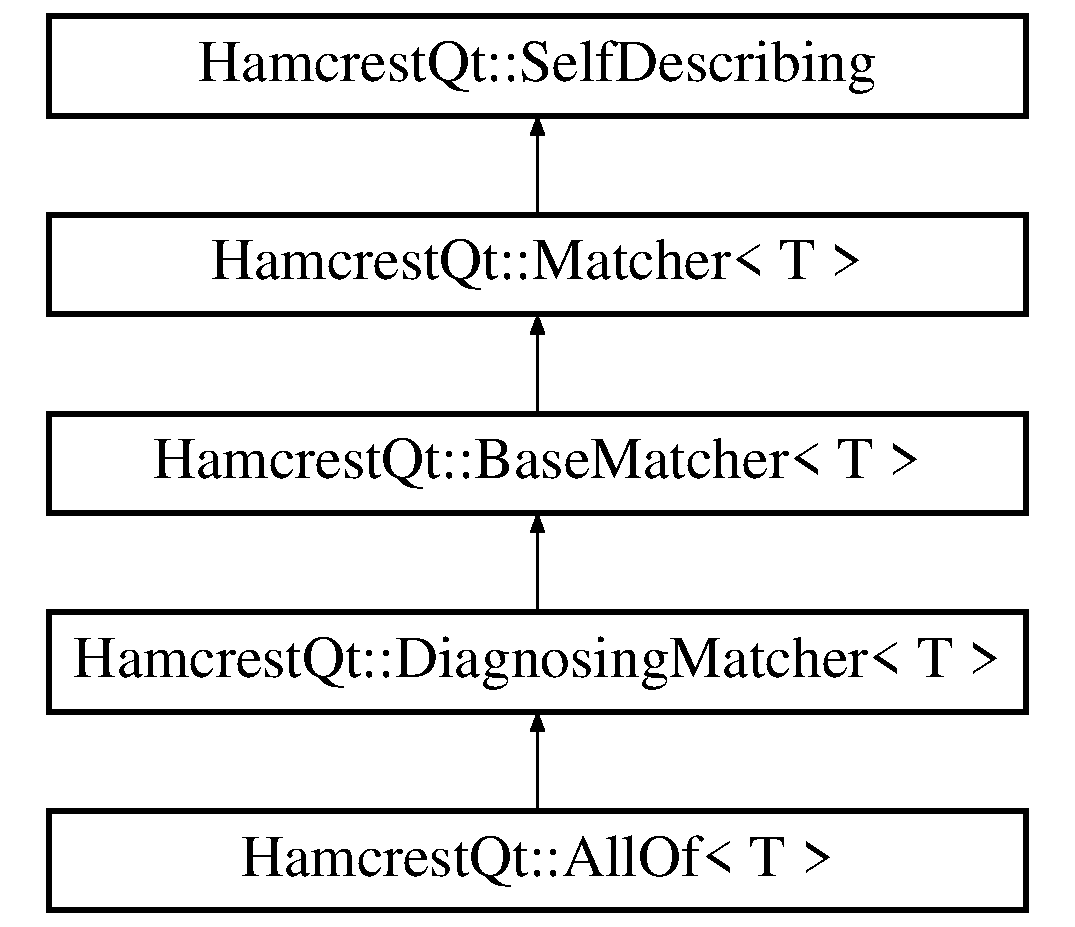
\includegraphics[height=5.000000cm]{class_hamcrest_qt_1_1_all_of}
\end{center}
\end{figure}
\subsection*{Public Member Functions}
\begin{DoxyCompactItemize}
\item 
\hypertarget{class_hamcrest_qt_1_1_all_of_a6bcbdedcab92058e3581b82672da354e}{{\bfseries All\-Of} (const Q\-List$<$ Q\-Shared\-Pointer$<$ \hyperlink{class_hamcrest_qt_1_1_matcher}{Matcher}$<$ T $>$ $>$ $>$ \&m)}\label{class_hamcrest_qt_1_1_all_of_a6bcbdedcab92058e3581b82672da354e}

\item 
\hypertarget{class_hamcrest_qt_1_1_all_of_ab912069c91c35566bff1d03777d98cd1}{virtual bool {\bfseries matches} (const T \&item, \hyperlink{class_hamcrest_qt_1_1_description}{Description} \&mismatch) const }\label{class_hamcrest_qt_1_1_all_of_ab912069c91c35566bff1d03777d98cd1}

\item 
virtual void \hyperlink{class_hamcrest_qt_1_1_all_of_a0b60757a18e9dc9e9dfd2582cda9d39d}{describe\-To} (\hyperlink{class_hamcrest_qt_1_1_description}{Description} \&description) const 
\begin{DoxyCompactList}\small\item\em Generates a description of the object. \end{DoxyCompactList}\end{DoxyCompactItemize}
\subsection*{Additional Inherited Members}


\subsection{Detailed Description}
\subsubsection*{template$<$typename T$>$class Hamcrest\-Qt\-::\-All\-Of$<$ T $>$}

Calculates the logical conjunction of multiple matchers. 

Evaluation is shortcut, so subsequent matchers are not called if an earlier matcher returns {\ttfamily false}. 

\subsection{Member Function Documentation}
\hypertarget{class_hamcrest_qt_1_1_all_of_a0b60757a18e9dc9e9dfd2582cda9d39d}{\index{Hamcrest\-Qt\-::\-All\-Of@{Hamcrest\-Qt\-::\-All\-Of}!describe\-To@{describe\-To}}
\index{describe\-To@{describe\-To}!HamcrestQt::AllOf@{Hamcrest\-Qt\-::\-All\-Of}}
\subsubsection[{describe\-To}]{\setlength{\rightskip}{0pt plus 5cm}template$<$typename T $>$ virtual void {\bf Hamcrest\-Qt\-::\-All\-Of}$<$ T $>$\-::describe\-To (
\begin{DoxyParamCaption}
\item[{{\bf Description} \&}]{description}
\end{DoxyParamCaption}
) const\hspace{0.3cm}{\ttfamily [inline]}, {\ttfamily [virtual]}}}\label{class_hamcrest_qt_1_1_all_of_a0b60757a18e9dc9e9dfd2582cda9d39d}


Generates a description of the object. 

The description may be part of a description of a larger object of which this is just a component, so it should be worded appropriately.


\begin{DoxyParams}{Parameters}
{\em description} & The description to be built or appended to. \\
\hline
\end{DoxyParams}


Implements \hyperlink{class_hamcrest_qt_1_1_self_describing_af04da98570148e5e943e42399f718e4c}{Hamcrest\-Qt\-::\-Self\-Describing}.



The documentation for this class was generated from the following file\-:\begin{DoxyCompactItemize}
\item 
C\-:/\-Users/\-Christian/\-Documents/\-Git\-Hub/\-Hamcrest-\/\-Qt/src/core/matcher/allof.\-h\end{DoxyCompactItemize}

\hypertarget{class_hamcrest_qt_1_1_any_of}{\section{Hamcrest\-Qt\-:\-:Any\-Of$<$ T $>$ Class Template Reference}
\label{class_hamcrest_qt_1_1_any_of}\index{Hamcrest\-Qt\-::\-Any\-Of$<$ T $>$@{Hamcrest\-Qt\-::\-Any\-Of$<$ T $>$}}
}


Calculates the logical disjunction of multiple matchers.  




{\ttfamily \#include $<$anyof.\-h$>$}

Inheritance diagram for Hamcrest\-Qt\-:\-:Any\-Of$<$ T $>$\-:\begin{figure}[H]
\begin{center}
\leavevmode
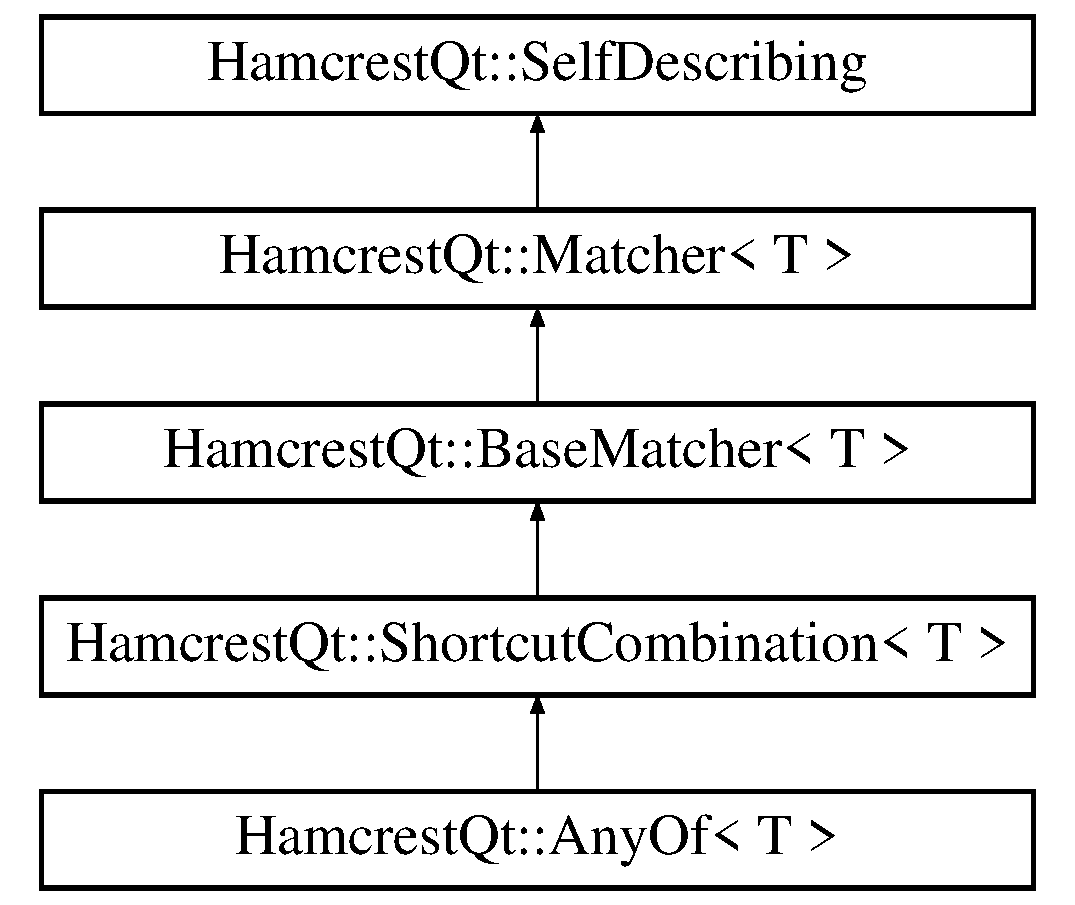
\includegraphics[height=5.000000cm]{class_hamcrest_qt_1_1_any_of}
\end{center}
\end{figure}
\subsection*{Public Member Functions}
\begin{DoxyCompactItemize}
\item 
\hypertarget{class_hamcrest_qt_1_1_any_of_a7dc9177bd13e2b0aa5ce221e3d2587f5}{{\bfseries Any\-Of} (const Q\-List$<$ Q\-Shared\-Pointer$<$ \hyperlink{class_hamcrest_qt_1_1_matcher}{Matcher}$<$ T $>$ $>$ $>$ \&m)}\label{class_hamcrest_qt_1_1_any_of_a7dc9177bd13e2b0aa5ce221e3d2587f5}

\item 
virtual bool \hyperlink{class_hamcrest_qt_1_1_any_of_aa097e760ed6ce642c1ee40c73d73bdce}{matches} (const T \&item) const 
\begin{DoxyCompactList}\small\item\em Evaluates the matcher for argument {\itshape item}. \end{DoxyCompactList}\item 
virtual void \hyperlink{class_hamcrest_qt_1_1_any_of_a32a386c0a8f6bab40344199964c3d62f}{describe\-To} (\hyperlink{class_hamcrest_qt_1_1_description}{Description} \&description) const 
\begin{DoxyCompactList}\small\item\em Generates a description of the object. \end{DoxyCompactList}\end{DoxyCompactItemize}
\subsection*{Additional Inherited Members}


\subsection{Detailed Description}
\subsubsection*{template$<$typename T$>$class Hamcrest\-Qt\-::\-Any\-Of$<$ T $>$}

Calculates the logical disjunction of multiple matchers. 

Evaluation is shortcut, so subsequent matchers are not called if an earlier matcher returns {\ttfamily true}. 

\subsection{Member Function Documentation}
\hypertarget{class_hamcrest_qt_1_1_any_of_a32a386c0a8f6bab40344199964c3d62f}{\index{Hamcrest\-Qt\-::\-Any\-Of@{Hamcrest\-Qt\-::\-Any\-Of}!describe\-To@{describe\-To}}
\index{describe\-To@{describe\-To}!HamcrestQt::AnyOf@{Hamcrest\-Qt\-::\-Any\-Of}}
\subsubsection[{describe\-To}]{\setlength{\rightskip}{0pt plus 5cm}template$<$typename T $>$ virtual void {\bf Hamcrest\-Qt\-::\-Any\-Of}$<$ T $>$\-::describe\-To (
\begin{DoxyParamCaption}
\item[{{\bf Description} \&}]{description}
\end{DoxyParamCaption}
) const\hspace{0.3cm}{\ttfamily [inline]}, {\ttfamily [virtual]}}}\label{class_hamcrest_qt_1_1_any_of_a32a386c0a8f6bab40344199964c3d62f}


Generates a description of the object. 

The description may be part of a description of a larger object of which this is just a component, so it should be worded appropriately.


\begin{DoxyParams}{Parameters}
{\em description} & The description to be built or appended to. \\
\hline
\end{DoxyParams}


Implements \hyperlink{class_hamcrest_qt_1_1_self_describing_af04da98570148e5e943e42399f718e4c}{Hamcrest\-Qt\-::\-Self\-Describing}.

\hypertarget{class_hamcrest_qt_1_1_any_of_aa097e760ed6ce642c1ee40c73d73bdce}{\index{Hamcrest\-Qt\-::\-Any\-Of@{Hamcrest\-Qt\-::\-Any\-Of}!matches@{matches}}
\index{matches@{matches}!HamcrestQt::AnyOf@{Hamcrest\-Qt\-::\-Any\-Of}}
\subsubsection[{matches}]{\setlength{\rightskip}{0pt plus 5cm}template$<$typename T $>$ virtual bool {\bf Hamcrest\-Qt\-::\-Any\-Of}$<$ T $>$\-::matches (
\begin{DoxyParamCaption}
\item[{const T \&}]{item}
\end{DoxyParamCaption}
) const\hspace{0.3cm}{\ttfamily [inline]}, {\ttfamily [virtual]}}}\label{class_hamcrest_qt_1_1_any_of_aa097e760ed6ce642c1ee40c73d73bdce}


Evaluates the matcher for argument {\itshape item}. 


\begin{DoxyParams}{Parameters}
{\em item} & the object against which the matcher is evaluated. \\
\hline
\end{DoxyParams}
\begin{DoxyReturn}{Returns}
{\ttfamily true} if {\itshape item} matches, otherwise {\ttfamily false}.
\end{DoxyReturn}
\begin{DoxySeeAlso}{See Also}
\hyperlink{class_hamcrest_qt_1_1_base_matcher}{Base\-Matcher} 
\end{DoxySeeAlso}


Implements \hyperlink{class_hamcrest_qt_1_1_matcher_a9a8a775345afd0fde8942a0755303075}{Hamcrest\-Qt\-::\-Matcher$<$ T $>$}.



The documentation for this class was generated from the following file\-:\begin{DoxyCompactItemize}
\item 
C\-:/\-Users/\-Christian/\-Documents/\-Git\-Hub/\-Hamcrest-\/\-Qt/src/core/matcher/anyof.\-h\end{DoxyCompactItemize}

\hypertarget{class_hamcrest_qt_1_1_matcher_assert_1_1_assertion_listener}{\section{Hamcrest\-Qt\-:\-:Matcher\-Assert\-:\-:Assertion\-Listener Class Reference}
\label{class_hamcrest_qt_1_1_matcher_assert_1_1_assertion_listener}\index{Hamcrest\-Qt\-::\-Matcher\-Assert\-::\-Assertion\-Listener@{Hamcrest\-Qt\-::\-Matcher\-Assert\-::\-Assertion\-Listener}}
}
\subsection*{Public Member Functions}
\begin{DoxyCompactItemize}
\item 
\hypertarget{class_hamcrest_qt_1_1_matcher_assert_1_1_assertion_listener_a3b4340dac131adf094dc786d11d3554e}{virtual void {\bfseries assertion\-Error} (const Q\-String \&message)=0}\label{class_hamcrest_qt_1_1_matcher_assert_1_1_assertion_listener_a3b4340dac131adf094dc786d11d3554e}

\end{DoxyCompactItemize}


The documentation for this class was generated from the following file\-:\begin{DoxyCompactItemize}
\item 
C\-:/\-Users/\-Christian/\-Documents/\-Git\-Hub/\-Hamcrest-\/\-Qt/src/core/matcherassert.\-h\end{DoxyCompactItemize}

\hypertarget{class_hamcrest_qt_1_1_base_description}{\section{Hamcrest\-Qt\-:\-:Base\-Description Class Reference}
\label{class_hamcrest_qt_1_1_base_description}\index{Hamcrest\-Qt\-::\-Base\-Description@{Hamcrest\-Qt\-::\-Base\-Description}}
}


A \hyperlink{class_hamcrest_qt_1_1_description}{Description} that is stored as a string.  




{\ttfamily \#include $<$basedescription.\-h$>$}

Inheritance diagram for Hamcrest\-Qt\-:\-:Base\-Description\-:\begin{figure}[H]
\begin{center}
\leavevmode
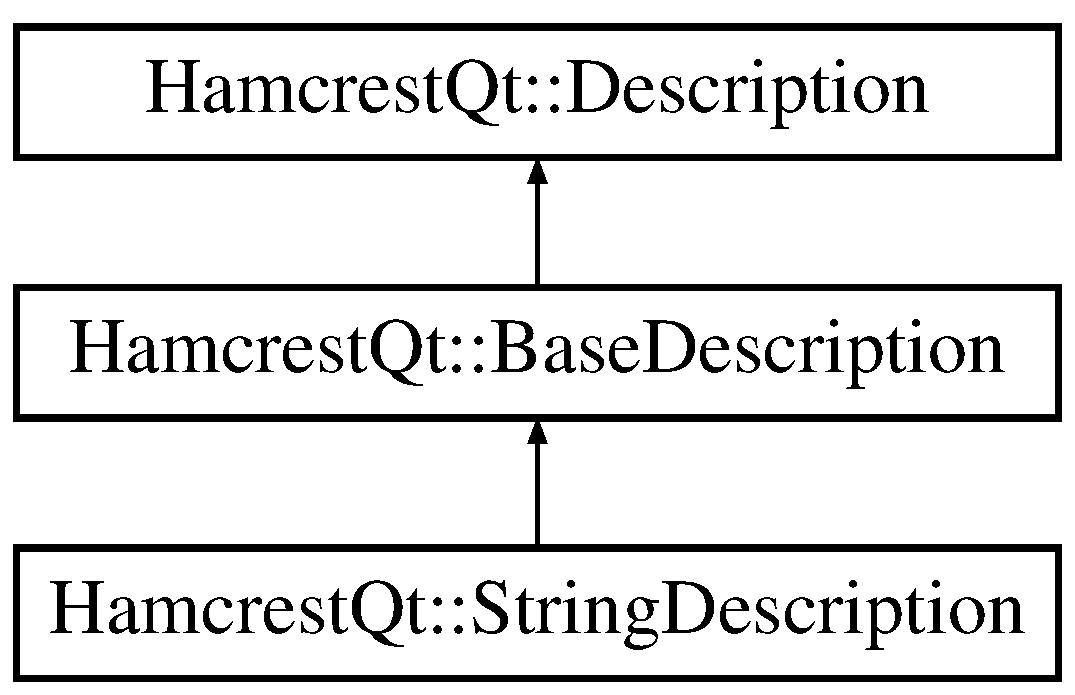
\includegraphics[height=3.000000cm]{class_hamcrest_qt_1_1_base_description}
\end{center}
\end{figure}
\subsection*{Public Member Functions}
\begin{DoxyCompactItemize}
\item 
\hypertarget{class_hamcrest_qt_1_1_base_description_a31de838e1dc68a94d60488cacbf2f1f8}{virtual \hyperlink{class_hamcrest_qt_1_1_description}{Description} \& \hyperlink{class_hamcrest_qt_1_1_base_description_a31de838e1dc68a94d60488cacbf2f1f8}{append\-Text} (const Q\-String \&text)}\label{class_hamcrest_qt_1_1_base_description_a31de838e1dc68a94d60488cacbf2f1f8}

\begin{DoxyCompactList}\small\item\em Appends some plain text to the description. \end{DoxyCompactList}\item 
\hypertarget{class_hamcrest_qt_1_1_base_description_a7ee8f64ba57295fa47dbda5946c875a2}{virtual \hyperlink{class_hamcrest_qt_1_1_description}{Description} \& \hyperlink{class_hamcrest_qt_1_1_base_description_a7ee8f64ba57295fa47dbda5946c875a2}{append\-Description\-Of} (const \hyperlink{class_hamcrest_qt_1_1_self_describing}{Self\-Describing} \&value)}\label{class_hamcrest_qt_1_1_base_description_a7ee8f64ba57295fa47dbda5946c875a2}

\begin{DoxyCompactList}\small\item\em Appends the description of a \hyperlink{class_hamcrest_qt_1_1_self_describing}{Self\-Describing} value to this description. \end{DoxyCompactList}\item 
\hypertarget{class_hamcrest_qt_1_1_base_description_acbf4636e7be54e338de55b182acd6b8c}{virtual Q\-String \hyperlink{class_hamcrest_qt_1_1_base_description_acbf4636e7be54e338de55b182acd6b8c}{to\-String} () const }\label{class_hamcrest_qt_1_1_base_description_acbf4636e7be54e338de55b182acd6b8c}

\begin{DoxyCompactList}\small\item\em Converts the description into a {\ttfamily Q\-String} value. \end{DoxyCompactList}\end{DoxyCompactItemize}
\subsection*{Protected Member Functions}
\begin{DoxyCompactItemize}
\item 
virtual void \hyperlink{class_hamcrest_qt_1_1_base_description_a7bb209dee8a47c3b4346a8126d0f0b3c}{append\-String} (const Q\-String \&str)
\begin{DoxyCompactList}\small\item\em Append the String {\itshape str} to the description. \end{DoxyCompactList}\end{DoxyCompactItemize}
\subsection*{Additional Inherited Members}


\subsection{Detailed Description}
A \hyperlink{class_hamcrest_qt_1_1_description}{Description} that is stored as a string. 

\subsection{Member Function Documentation}
\hypertarget{class_hamcrest_qt_1_1_base_description_a7bb209dee8a47c3b4346a8126d0f0b3c}{\index{Hamcrest\-Qt\-::\-Base\-Description@{Hamcrest\-Qt\-::\-Base\-Description}!append\-String@{append\-String}}
\index{append\-String@{append\-String}!HamcrestQt::BaseDescription@{Hamcrest\-Qt\-::\-Base\-Description}}
\subsubsection[{append\-String}]{\setlength{\rightskip}{0pt plus 5cm}void Hamcrest\-Qt\-::\-Base\-Description\-::append\-String (
\begin{DoxyParamCaption}
\item[{const Q\-String \&}]{str}
\end{DoxyParamCaption}
)\hspace{0.3cm}{\ttfamily [protected]}, {\ttfamily [virtual]}}}\label{class_hamcrest_qt_1_1_base_description_a7bb209dee8a47c3b4346a8126d0f0b3c}


Append the String {\itshape str} to the description. 

The default implementation passes every character to \hyperlink{}{append(\-Q\-Char)}. Override in subclasses to provide an efficient implementation. 

Implements \hyperlink{class_hamcrest_qt_1_1_description}{Hamcrest\-Qt\-::\-Description}.



Reimplemented in \hyperlink{class_hamcrest_qt_1_1_string_description_a2e27da55b34506521df58b3e2f22a48c}{Hamcrest\-Qt\-::\-String\-Description}.



The documentation for this class was generated from the following files\-:\begin{DoxyCompactItemize}
\item 
C\-:/\-Users/\-Christian/\-Documents/\-Git\-Hub/\-Hamcrest-\/\-Qt/src/core/basedescription.\-h\item 
C\-:/\-Users/\-Christian/\-Documents/\-Git\-Hub/\-Hamcrest-\/\-Qt/src/core/basedescription.\-cpp\end{DoxyCompactItemize}

\hypertarget{class_hamcrest_qt_1_1_base_matcher}{\section{Hamcrest\-Qt\-:\-:Base\-Matcher$<$ T $>$ Class Template Reference}
\label{class_hamcrest_qt_1_1_base_matcher}\index{Hamcrest\-Qt\-::\-Base\-Matcher$<$ T $>$@{Hamcrest\-Qt\-::\-Base\-Matcher$<$ T $>$}}
}


Base\-Class for all \hyperlink{class_hamcrest_qt_1_1_matcher}{Matcher} implementations.  




{\ttfamily \#include $<$basematcher.\-h$>$}

Inheritance diagram for Hamcrest\-Qt\-:\-:Base\-Matcher$<$ T $>$\-:\begin{figure}[H]
\begin{center}
\leavevmode
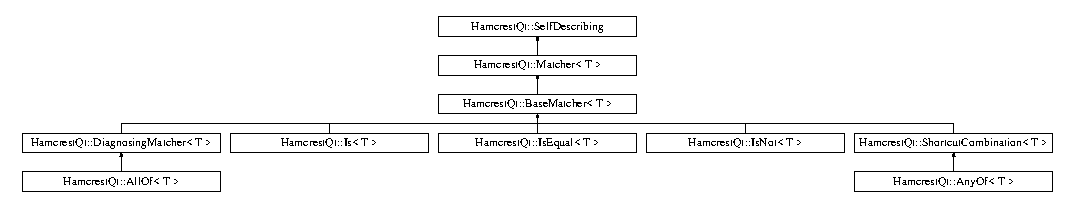
\includegraphics[height=2.343096cm]{class_hamcrest_qt_1_1_base_matcher}
\end{center}
\end{figure}
\subsection*{Public Member Functions}
\begin{DoxyCompactItemize}
\item 
virtual void \hyperlink{class_hamcrest_qt_1_1_base_matcher_a4299e8a4358ff624fb857a3301dd1b73}{describe\-Mismatch} (const T \&item, \hyperlink{class_hamcrest_qt_1_1_description}{Description} \&description) const 
\begin{DoxyCompactList}\small\item\em Generate a description of why the matcher has not accepted the item. \end{DoxyCompactList}\item 
\hypertarget{class_hamcrest_qt_1_1_base_matcher_a8d28bd3b881fa3ebb2177771360328ed}{virtual Q\-String {\bfseries to\-String} () const }\label{class_hamcrest_qt_1_1_base_matcher_a8d28bd3b881fa3ebb2177771360328ed}

\end{DoxyCompactItemize}


\subsection{Detailed Description}
\subsubsection*{template$<$typename T$>$class Hamcrest\-Qt\-::\-Base\-Matcher$<$ T $>$}

Base\-Class for all \hyperlink{class_hamcrest_qt_1_1_matcher}{Matcher} implementations. 

\begin{DoxySeeAlso}{See Also}
\hyperlink{class_hamcrest_qt_1_1_matcher}{Matcher} 
\end{DoxySeeAlso}


\subsection{Member Function Documentation}
\hypertarget{class_hamcrest_qt_1_1_base_matcher_a4299e8a4358ff624fb857a3301dd1b73}{\index{Hamcrest\-Qt\-::\-Base\-Matcher@{Hamcrest\-Qt\-::\-Base\-Matcher}!describe\-Mismatch@{describe\-Mismatch}}
\index{describe\-Mismatch@{describe\-Mismatch}!HamcrestQt::BaseMatcher@{Hamcrest\-Qt\-::\-Base\-Matcher}}
\subsubsection[{describe\-Mismatch}]{\setlength{\rightskip}{0pt plus 5cm}template$<$typename T$>$ virtual void {\bf Hamcrest\-Qt\-::\-Base\-Matcher}$<$ T $>$\-::describe\-Mismatch (
\begin{DoxyParamCaption}
\item[{const T \&}]{item, }
\item[{{\bf Description} \&}]{mismatch\-Description}
\end{DoxyParamCaption}
) const\hspace{0.3cm}{\ttfamily [inline]}, {\ttfamily [virtual]}}}\label{class_hamcrest_qt_1_1_base_matcher_a4299e8a4358ff624fb857a3301dd1b73}


Generate a description of why the matcher has not accepted the item. 

The description will be part of a larger description of why a matching failed, so it should be concise. This method assumes that {\ttfamily matches(item)} is false, but will not check this.


\begin{DoxyParams}{Parameters}
{\em item} & The item that the \hyperlink{class_hamcrest_qt_1_1_matcher}{Matcher} has rejected. \\
\hline
{\em mismatch\-Description} & The description to be built or appended to. \\
\hline
\end{DoxyParams}


Implements \hyperlink{class_hamcrest_qt_1_1_matcher_aa92292613ca3c83f0501d261de94cb2b}{Hamcrest\-Qt\-::\-Matcher$<$ T $>$}.



Reimplemented in \hyperlink{class_hamcrest_qt_1_1_is_a3a8c6b52b2b0636e24b60542359ba12e}{Hamcrest\-Qt\-::\-Is$<$ T $>$}, \hyperlink{class_hamcrest_qt_1_1_substring_matcher_a23bb6d4b756dd8745a883eb88a993a2b}{Hamcrest\-Qt\-::\-Substring\-Matcher}, and \hyperlink{class_hamcrest_qt_1_1_diagnosing_matcher_a122cccc22b8be886b3202e0a126995ed}{Hamcrest\-Qt\-::\-Diagnosing\-Matcher$<$ T $>$}.



The documentation for this class was generated from the following file\-:\begin{DoxyCompactItemize}
\item 
C\-:/\-Users/\-Christian/\-Documents/\-Git\-Hub/\-Hamcrest-\/\-Qt/src/core/basematcher.\-h\end{DoxyCompactItemize}

\hypertarget{class_hamcrest_qt_1_1_description}{\section{Hamcrest\-Qt\-:\-:Description Class Reference}
\label{class_hamcrest_qt_1_1_description}\index{Hamcrest\-Qt\-::\-Description@{Hamcrest\-Qt\-::\-Description}}
}


A description of a \hyperlink{class_hamcrest_qt_1_1_matcher}{Matcher}.  




{\ttfamily \#include $<$description.\-h$>$}

Inheritance diagram for Hamcrest\-Qt\-:\-:Description\-:\begin{figure}[H]
\begin{center}
\leavevmode
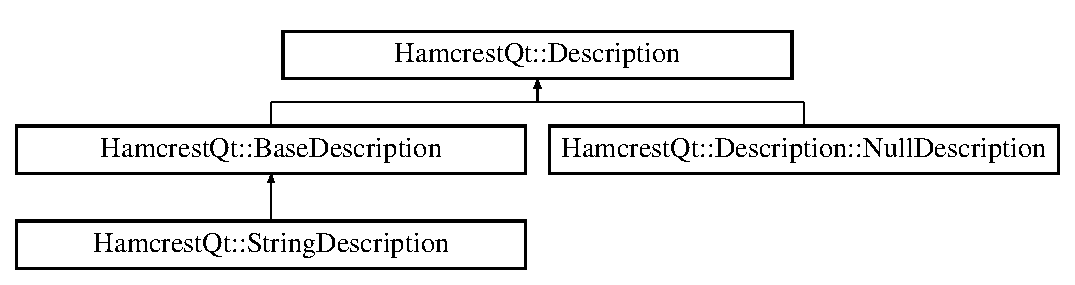
\includegraphics[height=3.000000cm]{class_hamcrest_qt_1_1_description}
\end{center}
\end{figure}
\subsection*{Classes}
\begin{DoxyCompactItemize}
\item 
class \hyperlink{class_hamcrest_qt_1_1_description_1_1_null_description}{Null\-Description}
\end{DoxyCompactItemize}
\subsection*{Public Member Functions}
\begin{DoxyCompactItemize}
\item 
\hypertarget{class_hamcrest_qt_1_1_description_ab6160a4dab7192858975de1827db2a63}{virtual \hyperlink{class_hamcrest_qt_1_1_description}{Description} \& \hyperlink{class_hamcrest_qt_1_1_description_ab6160a4dab7192858975de1827db2a63}{append\-Text} (const Q\-String \&text)=0}\label{class_hamcrest_qt_1_1_description_ab6160a4dab7192858975de1827db2a63}

\begin{DoxyCompactList}\small\item\em Appends some plain text to the description. \end{DoxyCompactList}\item 
\hypertarget{class_hamcrest_qt_1_1_description_a973e1c3f7ad1f782540a19404cb52c66}{virtual \hyperlink{class_hamcrest_qt_1_1_description}{Description} \& \hyperlink{class_hamcrest_qt_1_1_description_a973e1c3f7ad1f782540a19404cb52c66}{append\-Description\-Of} (const \hyperlink{class_hamcrest_qt_1_1_self_describing}{Self\-Describing} \&value)=0}\label{class_hamcrest_qt_1_1_description_a973e1c3f7ad1f782540a19404cb52c66}

\begin{DoxyCompactList}\small\item\em Appends the description of a \hyperlink{class_hamcrest_qt_1_1_self_describing}{Self\-Describing} value to this description. \end{DoxyCompactList}\item 
\hypertarget{class_hamcrest_qt_1_1_description_a4418ed4f68a03cf1b63b5875bf7ea65c}{{\footnotesize template$<$typename T $>$ }\\\hyperlink{class_hamcrest_qt_1_1_description}{Description} \& \hyperlink{class_hamcrest_qt_1_1_description_a4418ed4f68a03cf1b63b5875bf7ea65c}{append\-Value} (const T \&value)}\label{class_hamcrest_qt_1_1_description_a4418ed4f68a03cf1b63b5875bf7ea65c}

\begin{DoxyCompactList}\small\item\em Appends an arbitrary value to the description. \end{DoxyCompactList}\item 
\hypertarget{class_hamcrest_qt_1_1_description_a667e8d992135e9e0e55e5d8967e6eb9e}{\hyperlink{class_hamcrest_qt_1_1_description}{Description} \& {\bfseries append\-Value} (short value)}\label{class_hamcrest_qt_1_1_description_a667e8d992135e9e0e55e5d8967e6eb9e}

\item 
\hypertarget{class_hamcrest_qt_1_1_description_ad3194a1f9cb19c7ded63a9f4137a7a4f}{\hyperlink{class_hamcrest_qt_1_1_description}{Description} \& {\bfseries append\-Value} (long value)}\label{class_hamcrest_qt_1_1_description_ad3194a1f9cb19c7ded63a9f4137a7a4f}

\item 
\hypertarget{class_hamcrest_qt_1_1_description_a913cb1bed8a73253afb5277fa9057823}{\hyperlink{class_hamcrest_qt_1_1_description}{Description} \& {\bfseries append\-Value} (float value)}\label{class_hamcrest_qt_1_1_description_a913cb1bed8a73253afb5277fa9057823}

\item 
\hypertarget{class_hamcrest_qt_1_1_description_aac6bd98a42370398372e574f99d2dfa1}{\hyperlink{class_hamcrest_qt_1_1_description}{Description} \& {\bfseries append\-Value} (double value)}\label{class_hamcrest_qt_1_1_description_aac6bd98a42370398372e574f99d2dfa1}

\item 
\hypertarget{class_hamcrest_qt_1_1_description_a97cbeccfaf86284a12f7411194e627f3}{\hyperlink{class_hamcrest_qt_1_1_description}{Description} \& {\bfseries append\-Value} (const char $\ast$value)}\label{class_hamcrest_qt_1_1_description_a97cbeccfaf86284a12f7411194e627f3}

\item 
\hypertarget{class_hamcrest_qt_1_1_description_a3021527892a3d95ae5c060a758a39d5e}{\hyperlink{class_hamcrest_qt_1_1_description}{Description} \& {\bfseries append\-Value} (const Q\-String \&value)}\label{class_hamcrest_qt_1_1_description_a3021527892a3d95ae5c060a758a39d5e}

\item 
\hypertarget{class_hamcrest_qt_1_1_description_a1509fac2374ef729fc5e84dd37c43dc1}{\hyperlink{class_hamcrest_qt_1_1_description}{Description} \& {\bfseries append\-Value} (char value)}\label{class_hamcrest_qt_1_1_description_a1509fac2374ef729fc5e84dd37c43dc1}

\item 
\hypertarget{class_hamcrest_qt_1_1_description_a0df92a24ec9f68a7a711ef381fe9bb7a}{\hyperlink{class_hamcrest_qt_1_1_description}{Description} \& {\bfseries append\-Value} (const Q\-Char \&value)}\label{class_hamcrest_qt_1_1_description_a0df92a24ec9f68a7a711ef381fe9bb7a}

\item 
\hypertarget{class_hamcrest_qt_1_1_description_a7bb11eef4483ba18cdee9d04e8d6fdd7}{{\footnotesize template$<$typename Iterator $>$ }\\\hyperlink{class_hamcrest_qt_1_1_description}{Description} \& \hyperlink{class_hamcrest_qt_1_1_description_a7bb11eef4483ba18cdee9d04e8d6fdd7}{append\-List} (const Q\-String \&start, const Q\-String \&separator, const Q\-String \&end, Iterator start\-Iterator, Iterator end\-Iterator)}\label{class_hamcrest_qt_1_1_description_a7bb11eef4483ba18cdee9d04e8d6fdd7}

\begin{DoxyCompactList}\small\item\em Appends a list of \hyperlink{class_hamcrest_qt_1_1_self_describing}{Self\-Describing} objects to the description. \end{DoxyCompactList}\item 
\hypertarget{class_hamcrest_qt_1_1_description_aaee6521f18333eaeb4753099fa040116}{virtual Q\-String \hyperlink{class_hamcrest_qt_1_1_description_aaee6521f18333eaeb4753099fa040116}{to\-String} () const =0}\label{class_hamcrest_qt_1_1_description_aaee6521f18333eaeb4753099fa040116}

\begin{DoxyCompactList}\small\item\em Converts the description into a {\ttfamily Q\-String} value. \end{DoxyCompactList}\end{DoxyCompactItemize}
\subsection*{Static Public Member Functions}
\begin{DoxyCompactItemize}
\item 
\hypertarget{class_hamcrest_qt_1_1_description_a7f7e1276e3c41c890f83f147ddffad16}{static \hyperlink{class_hamcrest_qt_1_1_description}{Description} \& {\bfseries N\-O\-N\-E} ()}\label{class_hamcrest_qt_1_1_description_a7f7e1276e3c41c890f83f147ddffad16}

\end{DoxyCompactItemize}
\subsection*{Protected Member Functions}
\begin{DoxyCompactItemize}
\item 
\hypertarget{class_hamcrest_qt_1_1_description_a355744585a874de9ccd6bab303826a71}{virtual void {\bfseries append\-String} (const Q\-String \&str)=0}\label{class_hamcrest_qt_1_1_description_a355744585a874de9ccd6bab303826a71}

\item 
\hypertarget{class_hamcrest_qt_1_1_description_ad691e2adacec9d180ce13940e84e80c8}{virtual void {\bfseries append} (const Q\-Char \&c)=0}\label{class_hamcrest_qt_1_1_description_ad691e2adacec9d180ce13940e84e80c8}

\item 
\hypertarget{class_hamcrest_qt_1_1_description_a4bc07ffd801a681b3698aac5c3e2f79f}{virtual void {\bfseries to\-Cpp\-Syntax\-String} (const Q\-String \&unformatted)}\label{class_hamcrest_qt_1_1_description_a4bc07ffd801a681b3698aac5c3e2f79f}

\item 
\hypertarget{class_hamcrest_qt_1_1_description_a01bdce4a7500e30f997f78332521de36}{virtual void {\bfseries to\-Cpp\-Syntax} (const Q\-Char \&ch)}\label{class_hamcrest_qt_1_1_description_a01bdce4a7500e30f997f78332521de36}

\end{DoxyCompactItemize}


\subsection{Detailed Description}
A description of a \hyperlink{class_hamcrest_qt_1_1_matcher}{Matcher}. 

A \hyperlink{class_hamcrest_qt_1_1_matcher}{Matcher} will describe itself to a description which can later be used for reporting.

\begin{DoxySeeAlso}{See Also}
Matcher\-::describe\-To(\-Description) 
\end{DoxySeeAlso}


The documentation for this class was generated from the following files\-:\begin{DoxyCompactItemize}
\item 
C\-:/\-Users/\-Christian/\-Documents/\-Git\-Hub/\-Hamcrest-\/\-Qt/src/core/description.\-h\item 
C\-:/\-Users/\-Christian/\-Documents/\-Git\-Hub/\-Hamcrest-\/\-Qt/src/core/description.\-cpp\end{DoxyCompactItemize}

\hypertarget{class_hamcrest_qt_1_1_diagnosing_matcher}{\section{Hamcrest\-Qt\-:\-:Diagnosing\-Matcher$<$ T $>$ Class Template Reference}
\label{class_hamcrest_qt_1_1_diagnosing_matcher}\index{Hamcrest\-Qt\-::\-Diagnosing\-Matcher$<$ T $>$@{Hamcrest\-Qt\-::\-Diagnosing\-Matcher$<$ T $>$}}
}
Inheritance diagram for Hamcrest\-Qt\-:\-:Diagnosing\-Matcher$<$ T $>$\-:\begin{figure}[H]
\begin{center}
\leavevmode
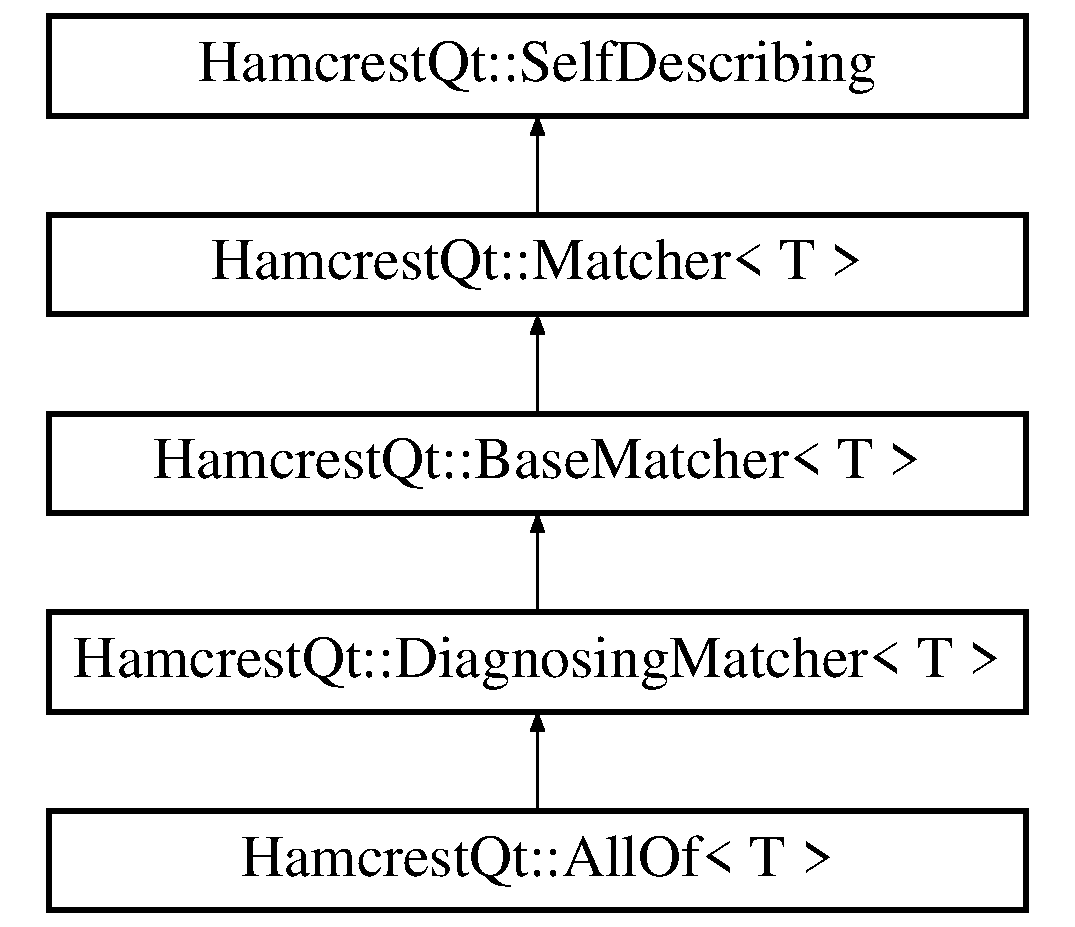
\includegraphics[height=5.000000cm]{class_hamcrest_qt_1_1_diagnosing_matcher}
\end{center}
\end{figure}
\subsection*{Public Member Functions}
\begin{DoxyCompactItemize}
\item 
virtual bool \hyperlink{class_hamcrest_qt_1_1_diagnosing_matcher_a95ea76988bacda59586ec1423c4d0e6c}{matches} (const T \&item) const 
\begin{DoxyCompactList}\small\item\em Evaluates the matcher for argument {\itshape item}. \end{DoxyCompactList}\item 
virtual void \hyperlink{class_hamcrest_qt_1_1_diagnosing_matcher_a122cccc22b8be886b3202e0a126995ed}{describe\-Mismatch} (const T \&item, \hyperlink{class_hamcrest_qt_1_1_description}{Description} \&mismatch\-Description) const 
\begin{DoxyCompactList}\small\item\em Generate a description of why the matcher has not accepted the item. \end{DoxyCompactList}\end{DoxyCompactItemize}
\subsection*{Protected Member Functions}
\begin{DoxyCompactItemize}
\item 
\hypertarget{class_hamcrest_qt_1_1_diagnosing_matcher_a7e4d9a805fe53502e44b8633f8618425}{virtual bool {\bfseries matches} (const T \&item, \hyperlink{class_hamcrest_qt_1_1_description}{Description} \&mismatch\-Description) const =0}\label{class_hamcrest_qt_1_1_diagnosing_matcher_a7e4d9a805fe53502e44b8633f8618425}

\end{DoxyCompactItemize}


\subsection{Member Function Documentation}
\hypertarget{class_hamcrest_qt_1_1_diagnosing_matcher_a122cccc22b8be886b3202e0a126995ed}{\index{Hamcrest\-Qt\-::\-Diagnosing\-Matcher@{Hamcrest\-Qt\-::\-Diagnosing\-Matcher}!describe\-Mismatch@{describe\-Mismatch}}
\index{describe\-Mismatch@{describe\-Mismatch}!HamcrestQt::DiagnosingMatcher@{Hamcrest\-Qt\-::\-Diagnosing\-Matcher}}
\subsubsection[{describe\-Mismatch}]{\setlength{\rightskip}{0pt plus 5cm}template$<$typename T $>$ virtual void {\bf Hamcrest\-Qt\-::\-Diagnosing\-Matcher}$<$ T $>$\-::describe\-Mismatch (
\begin{DoxyParamCaption}
\item[{const T \&}]{item, }
\item[{{\bf Description} \&}]{mismatch\-Description}
\end{DoxyParamCaption}
) const\hspace{0.3cm}{\ttfamily [inline]}, {\ttfamily [virtual]}}}\label{class_hamcrest_qt_1_1_diagnosing_matcher_a122cccc22b8be886b3202e0a126995ed}


Generate a description of why the matcher has not accepted the item. 

The description will be part of a larger description of why a matching failed, so it should be concise. This method assumes that {\ttfamily matches(item)} is false, but will not check this.


\begin{DoxyParams}{Parameters}
{\em item} & The item that the \hyperlink{class_hamcrest_qt_1_1_matcher}{Matcher} has rejected. \\
\hline
{\em mismatch\-Description} & The description to be built or appended to. \\
\hline
\end{DoxyParams}


Reimplemented from \hyperlink{class_hamcrest_qt_1_1_base_matcher_a4299e8a4358ff624fb857a3301dd1b73}{Hamcrest\-Qt\-::\-Base\-Matcher$<$ T $>$}.

\hypertarget{class_hamcrest_qt_1_1_diagnosing_matcher_a95ea76988bacda59586ec1423c4d0e6c}{\index{Hamcrest\-Qt\-::\-Diagnosing\-Matcher@{Hamcrest\-Qt\-::\-Diagnosing\-Matcher}!matches@{matches}}
\index{matches@{matches}!HamcrestQt::DiagnosingMatcher@{Hamcrest\-Qt\-::\-Diagnosing\-Matcher}}
\subsubsection[{matches}]{\setlength{\rightskip}{0pt plus 5cm}template$<$typename T $>$ virtual bool {\bf Hamcrest\-Qt\-::\-Diagnosing\-Matcher}$<$ T $>$\-::matches (
\begin{DoxyParamCaption}
\item[{const T \&}]{item}
\end{DoxyParamCaption}
) const\hspace{0.3cm}{\ttfamily [inline]}, {\ttfamily [virtual]}}}\label{class_hamcrest_qt_1_1_diagnosing_matcher_a95ea76988bacda59586ec1423c4d0e6c}


Evaluates the matcher for argument {\itshape item}. 


\begin{DoxyParams}{Parameters}
{\em item} & the object against which the matcher is evaluated. \\
\hline
\end{DoxyParams}
\begin{DoxyReturn}{Returns}
{\ttfamily true} if {\itshape item} matches, otherwise {\ttfamily false}.
\end{DoxyReturn}
\begin{DoxySeeAlso}{See Also}
\hyperlink{class_hamcrest_qt_1_1_base_matcher}{Base\-Matcher} 
\end{DoxySeeAlso}


Implements \hyperlink{class_hamcrest_qt_1_1_matcher_a9a8a775345afd0fde8942a0755303075}{Hamcrest\-Qt\-::\-Matcher$<$ T $>$}.



The documentation for this class was generated from the following file\-:\begin{DoxyCompactItemize}
\item 
C\-:/\-Users/\-Christian/\-Documents/\-Git\-Hub/\-Hamcrest-\/\-Qt/src/core/diagnosingmatcher.\-h\end{DoxyCompactItemize}

\hypertarget{class_hamcrest_qt_1_1_is}{\section{Hamcrest\-Qt\-:\-:Is$<$ T $>$ Class Template Reference}
\label{class_hamcrest_qt_1_1_is}\index{Hamcrest\-Qt\-::\-Is$<$ T $>$@{Hamcrest\-Qt\-::\-Is$<$ T $>$}}
}


Decorates another \hyperlink{class_hamcrest_qt_1_1_matcher}{Matcher}, retaining the behaviour but allowing tests to be slightly more expressive.  




{\ttfamily \#include $<$is.\-h$>$}

Inheritance diagram for Hamcrest\-Qt\-:\-:Is$<$ T $>$\-:\begin{figure}[H]
\begin{center}
\leavevmode
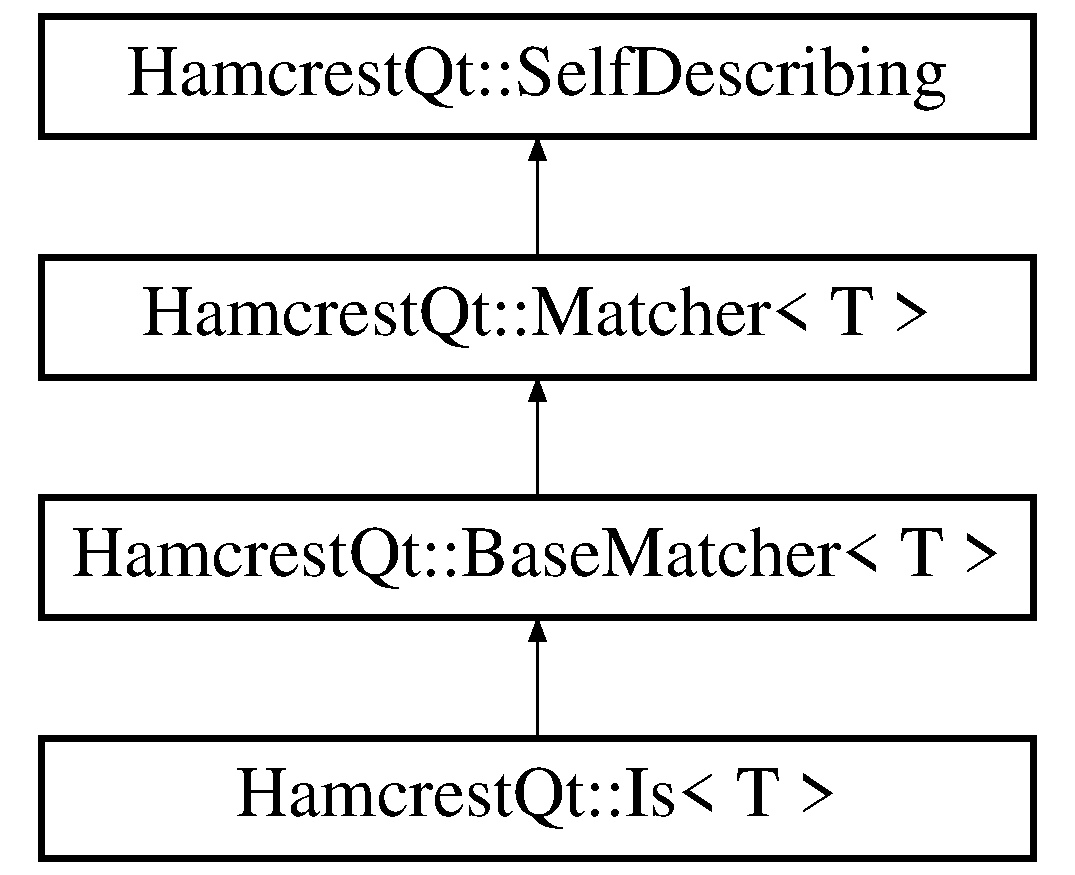
\includegraphics[height=4.000000cm]{class_hamcrest_qt_1_1_is}
\end{center}
\end{figure}
\subsection*{Public Member Functions}
\begin{DoxyCompactItemize}
\item 
\hypertarget{class_hamcrest_qt_1_1_is_aa2ab2ed0ac9f749371982ddc159806a2}{{\bfseries Is} (const Q\-Shared\-Pointer$<$ \hyperlink{class_hamcrest_qt_1_1_matcher}{Matcher}$<$ T $>$ $>$ \&m)}\label{class_hamcrest_qt_1_1_is_aa2ab2ed0ac9f749371982ddc159806a2}

\item 
virtual bool \hyperlink{class_hamcrest_qt_1_1_is_ab8ab441f01e21785134ec0bbfb53f0b4}{matches} (const T \&item) const 
\begin{DoxyCompactList}\small\item\em Evaluates the matcher for argument {\itshape item}. \end{DoxyCompactList}\item 
virtual void \hyperlink{class_hamcrest_qt_1_1_is_adcddba2f01e78feaff9f75ab3c5c7dd2}{describe\-To} (\hyperlink{class_hamcrest_qt_1_1_description}{Description} \&description) const 
\begin{DoxyCompactList}\small\item\em Generates a description of the object. \end{DoxyCompactList}\item 
virtual void \hyperlink{class_hamcrest_qt_1_1_is_a3a8c6b52b2b0636e24b60542359ba12e}{describe\-Mismatch} (const T \&item, \hyperlink{class_hamcrest_qt_1_1_description}{Description} \&description) const 
\begin{DoxyCompactList}\small\item\em Generate a description of why the matcher has not accepted the item. \end{DoxyCompactList}\end{DoxyCompactItemize}


\subsection{Detailed Description}
\subsubsection*{template$<$typename T$>$class Hamcrest\-Qt\-::\-Is$<$ T $>$}

Decorates another \hyperlink{class_hamcrest_qt_1_1_matcher}{Matcher}, retaining the behaviour but allowing tests to be slightly more expressive. 

For example\-: assert\-That(cheese, equal\-To(smelly)) vs. assert\-That(cheese, is(equal\-To(smelly))) 

\subsection{Member Function Documentation}
\hypertarget{class_hamcrest_qt_1_1_is_a3a8c6b52b2b0636e24b60542359ba12e}{\index{Hamcrest\-Qt\-::\-Is@{Hamcrest\-Qt\-::\-Is}!describe\-Mismatch@{describe\-Mismatch}}
\index{describe\-Mismatch@{describe\-Mismatch}!HamcrestQt::Is@{Hamcrest\-Qt\-::\-Is}}
\subsubsection[{describe\-Mismatch}]{\setlength{\rightskip}{0pt plus 5cm}template$<$typename T $>$ virtual void {\bf Hamcrest\-Qt\-::\-Is}$<$ T $>$\-::describe\-Mismatch (
\begin{DoxyParamCaption}
\item[{const T \&}]{item, }
\item[{{\bf Description} \&}]{mismatch\-Description}
\end{DoxyParamCaption}
) const\hspace{0.3cm}{\ttfamily [inline]}, {\ttfamily [virtual]}}}\label{class_hamcrest_qt_1_1_is_a3a8c6b52b2b0636e24b60542359ba12e}


Generate a description of why the matcher has not accepted the item. 

The description will be part of a larger description of why a matching failed, so it should be concise. This method assumes that {\ttfamily matches(item)} is false, but will not check this.


\begin{DoxyParams}{Parameters}
{\em item} & The item that the \hyperlink{class_hamcrest_qt_1_1_matcher}{Matcher} has rejected. \\
\hline
{\em mismatch\-Description} & The description to be built or appended to. \\
\hline
\end{DoxyParams}


Reimplemented from \hyperlink{class_hamcrest_qt_1_1_base_matcher_a4299e8a4358ff624fb857a3301dd1b73}{Hamcrest\-Qt\-::\-Base\-Matcher$<$ T $>$}.

\hypertarget{class_hamcrest_qt_1_1_is_adcddba2f01e78feaff9f75ab3c5c7dd2}{\index{Hamcrest\-Qt\-::\-Is@{Hamcrest\-Qt\-::\-Is}!describe\-To@{describe\-To}}
\index{describe\-To@{describe\-To}!HamcrestQt::Is@{Hamcrest\-Qt\-::\-Is}}
\subsubsection[{describe\-To}]{\setlength{\rightskip}{0pt plus 5cm}template$<$typename T $>$ virtual void {\bf Hamcrest\-Qt\-::\-Is}$<$ T $>$\-::describe\-To (
\begin{DoxyParamCaption}
\item[{{\bf Description} \&}]{description}
\end{DoxyParamCaption}
) const\hspace{0.3cm}{\ttfamily [inline]}, {\ttfamily [virtual]}}}\label{class_hamcrest_qt_1_1_is_adcddba2f01e78feaff9f75ab3c5c7dd2}


Generates a description of the object. 

The description may be part of a description of a larger object of which this is just a component, so it should be worded appropriately.


\begin{DoxyParams}{Parameters}
{\em description} & The description to be built or appended to. \\
\hline
\end{DoxyParams}


Implements \hyperlink{class_hamcrest_qt_1_1_self_describing_af04da98570148e5e943e42399f718e4c}{Hamcrest\-Qt\-::\-Self\-Describing}.

\hypertarget{class_hamcrest_qt_1_1_is_ab8ab441f01e21785134ec0bbfb53f0b4}{\index{Hamcrest\-Qt\-::\-Is@{Hamcrest\-Qt\-::\-Is}!matches@{matches}}
\index{matches@{matches}!HamcrestQt::Is@{Hamcrest\-Qt\-::\-Is}}
\subsubsection[{matches}]{\setlength{\rightskip}{0pt plus 5cm}template$<$typename T $>$ virtual bool {\bf Hamcrest\-Qt\-::\-Is}$<$ T $>$\-::matches (
\begin{DoxyParamCaption}
\item[{const T \&}]{item}
\end{DoxyParamCaption}
) const\hspace{0.3cm}{\ttfamily [inline]}, {\ttfamily [virtual]}}}\label{class_hamcrest_qt_1_1_is_ab8ab441f01e21785134ec0bbfb53f0b4}


Evaluates the matcher for argument {\itshape item}. 


\begin{DoxyParams}{Parameters}
{\em item} & the object against which the matcher is evaluated. \\
\hline
\end{DoxyParams}
\begin{DoxyReturn}{Returns}
{\ttfamily true} if {\itshape item} matches, otherwise {\ttfamily false}.
\end{DoxyReturn}
\begin{DoxySeeAlso}{See Also}
\hyperlink{class_hamcrest_qt_1_1_base_matcher}{Base\-Matcher} 
\end{DoxySeeAlso}


Implements \hyperlink{class_hamcrest_qt_1_1_matcher_a9a8a775345afd0fde8942a0755303075}{Hamcrest\-Qt\-::\-Matcher$<$ T $>$}.



The documentation for this class was generated from the following file\-:\begin{DoxyCompactItemize}
\item 
C\-:/\-Users/\-Christian/\-Documents/\-Git\-Hub/\-Hamcrest-\/\-Qt/src/core/matcher/is.\-h\end{DoxyCompactItemize}

\hypertarget{class_hamcrest_qt_1_1_is_equal}{\section{Hamcrest\-Qt\-:\-:Is\-Equal$<$ T $>$ Class Template Reference}
\label{class_hamcrest_qt_1_1_is_equal}\index{Hamcrest\-Qt\-::\-Is\-Equal$<$ T $>$@{Hamcrest\-Qt\-::\-Is\-Equal$<$ T $>$}}
}


\hyperlink{class_hamcrest_qt_1_1_is}{Is} the value equal to another value, as tested by the operator==() method?  




{\ttfamily \#include $<$isequal.\-h$>$}

Inheritance diagram for Hamcrest\-Qt\-:\-:Is\-Equal$<$ T $>$\-:\begin{figure}[H]
\begin{center}
\leavevmode
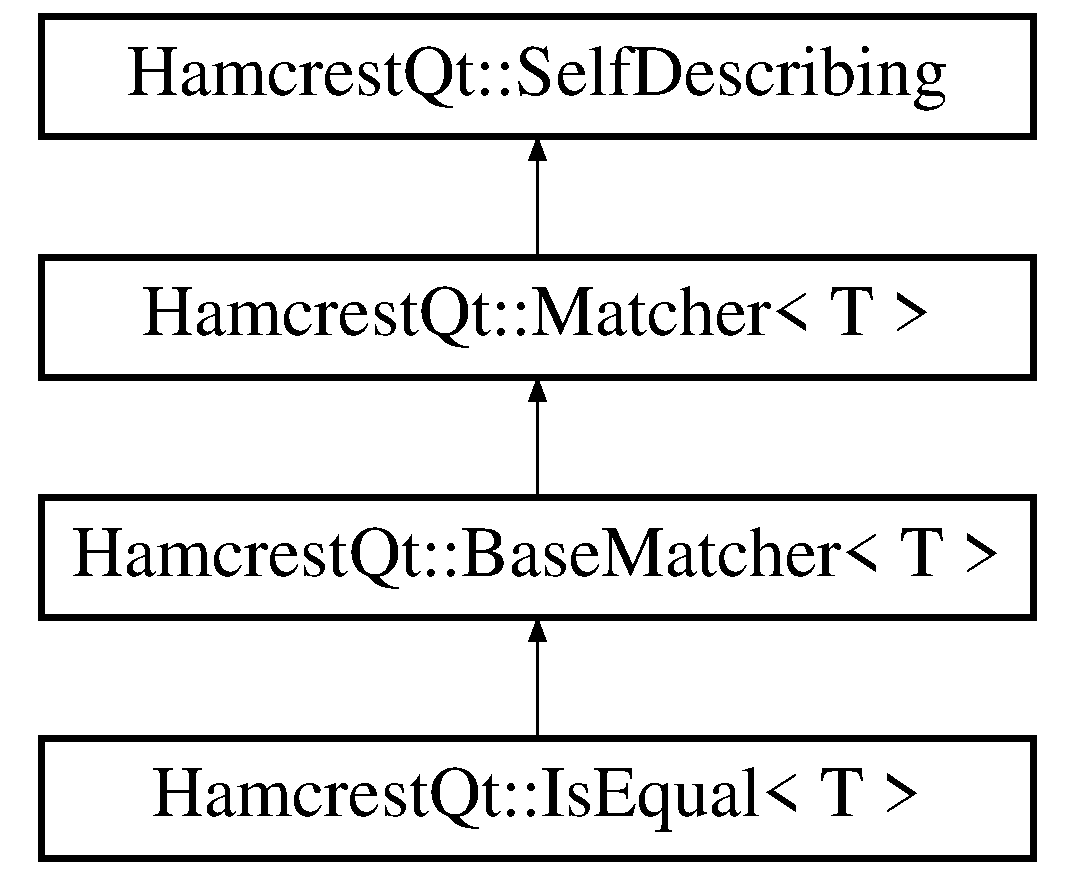
\includegraphics[height=4.000000cm]{class_hamcrest_qt_1_1_is_equal}
\end{center}
\end{figure}
\subsection*{Public Member Functions}
\begin{DoxyCompactItemize}
\item 
\hypertarget{class_hamcrest_qt_1_1_is_equal_a4c0ff1098477674f9a510eff0df01eb0}{{\bfseries Is\-Equal} (const T \&equal\-Arg)}\label{class_hamcrest_qt_1_1_is_equal_a4c0ff1098477674f9a510eff0df01eb0}

\item 
virtual bool \hyperlink{class_hamcrest_qt_1_1_is_equal_a4a9cc0239c034328baa5aeedf340271f}{matches} (const T \&actual\-Value) const 
\begin{DoxyCompactList}\small\item\em Evaluates the matcher for argument {\itshape item}. \end{DoxyCompactList}\item 
virtual void \hyperlink{class_hamcrest_qt_1_1_is_equal_a0f8431cbae42ab84f803c33eb43af260}{describe\-To} (\hyperlink{class_hamcrest_qt_1_1_description}{Description} \&description) const 
\begin{DoxyCompactList}\small\item\em Generates a description of the object. \end{DoxyCompactList}\end{DoxyCompactItemize}


\subsection{Detailed Description}
\subsubsection*{template$<$typename T$>$class Hamcrest\-Qt\-::\-Is\-Equal$<$ T $>$}

\hyperlink{class_hamcrest_qt_1_1_is}{Is} the value equal to another value, as tested by the operator==() method? 

\subsection{Member Function Documentation}
\hypertarget{class_hamcrest_qt_1_1_is_equal_a0f8431cbae42ab84f803c33eb43af260}{\index{Hamcrest\-Qt\-::\-Is\-Equal@{Hamcrest\-Qt\-::\-Is\-Equal}!describe\-To@{describe\-To}}
\index{describe\-To@{describe\-To}!HamcrestQt::IsEqual@{Hamcrest\-Qt\-::\-Is\-Equal}}
\subsubsection[{describe\-To}]{\setlength{\rightskip}{0pt plus 5cm}template$<$typename T $>$ virtual void {\bf Hamcrest\-Qt\-::\-Is\-Equal}$<$ T $>$\-::describe\-To (
\begin{DoxyParamCaption}
\item[{{\bf Description} \&}]{description}
\end{DoxyParamCaption}
) const\hspace{0.3cm}{\ttfamily [inline]}, {\ttfamily [virtual]}}}\label{class_hamcrest_qt_1_1_is_equal_a0f8431cbae42ab84f803c33eb43af260}


Generates a description of the object. 

The description may be part of a description of a larger object of which this is just a component, so it should be worded appropriately.


\begin{DoxyParams}{Parameters}
{\em description} & The description to be built or appended to. \\
\hline
\end{DoxyParams}


Implements \hyperlink{class_hamcrest_qt_1_1_self_describing_af04da98570148e5e943e42399f718e4c}{Hamcrest\-Qt\-::\-Self\-Describing}.

\hypertarget{class_hamcrest_qt_1_1_is_equal_a4a9cc0239c034328baa5aeedf340271f}{\index{Hamcrest\-Qt\-::\-Is\-Equal@{Hamcrest\-Qt\-::\-Is\-Equal}!matches@{matches}}
\index{matches@{matches}!HamcrestQt::IsEqual@{Hamcrest\-Qt\-::\-Is\-Equal}}
\subsubsection[{matches}]{\setlength{\rightskip}{0pt plus 5cm}template$<$typename T $>$ virtual bool {\bf Hamcrest\-Qt\-::\-Is\-Equal}$<$ T $>$\-::matches (
\begin{DoxyParamCaption}
\item[{const T \&}]{item}
\end{DoxyParamCaption}
) const\hspace{0.3cm}{\ttfamily [inline]}, {\ttfamily [virtual]}}}\label{class_hamcrest_qt_1_1_is_equal_a4a9cc0239c034328baa5aeedf340271f}


Evaluates the matcher for argument {\itshape item}. 


\begin{DoxyParams}{Parameters}
{\em item} & the object against which the matcher is evaluated. \\
\hline
\end{DoxyParams}
\begin{DoxyReturn}{Returns}
{\ttfamily true} if {\itshape item} matches, otherwise {\ttfamily false}.
\end{DoxyReturn}
\begin{DoxySeeAlso}{See Also}
\hyperlink{class_hamcrest_qt_1_1_base_matcher}{Base\-Matcher} 
\end{DoxySeeAlso}


Implements \hyperlink{class_hamcrest_qt_1_1_matcher_a9a8a775345afd0fde8942a0755303075}{Hamcrest\-Qt\-::\-Matcher$<$ T $>$}.



The documentation for this class was generated from the following file\-:\begin{DoxyCompactItemize}
\item 
C\-:/\-Users/\-Christian/\-Documents/\-Git\-Hub/\-Hamcrest-\/\-Qt/src/core/matcher/isequal.\-h\end{DoxyCompactItemize}

\hypertarget{class_hamcrest_qt_1_1_is_not}{\section{Hamcrest\-Qt\-:\-:Is\-Not$<$ T $>$ Class Template Reference}
\label{class_hamcrest_qt_1_1_is_not}\index{Hamcrest\-Qt\-::\-Is\-Not$<$ T $>$@{Hamcrest\-Qt\-::\-Is\-Not$<$ T $>$}}
}


Calculates the logical negation of a matcher.  




{\ttfamily \#include $<$isnot.\-h$>$}

Inheritance diagram for Hamcrest\-Qt\-:\-:Is\-Not$<$ T $>$\-:\begin{figure}[H]
\begin{center}
\leavevmode
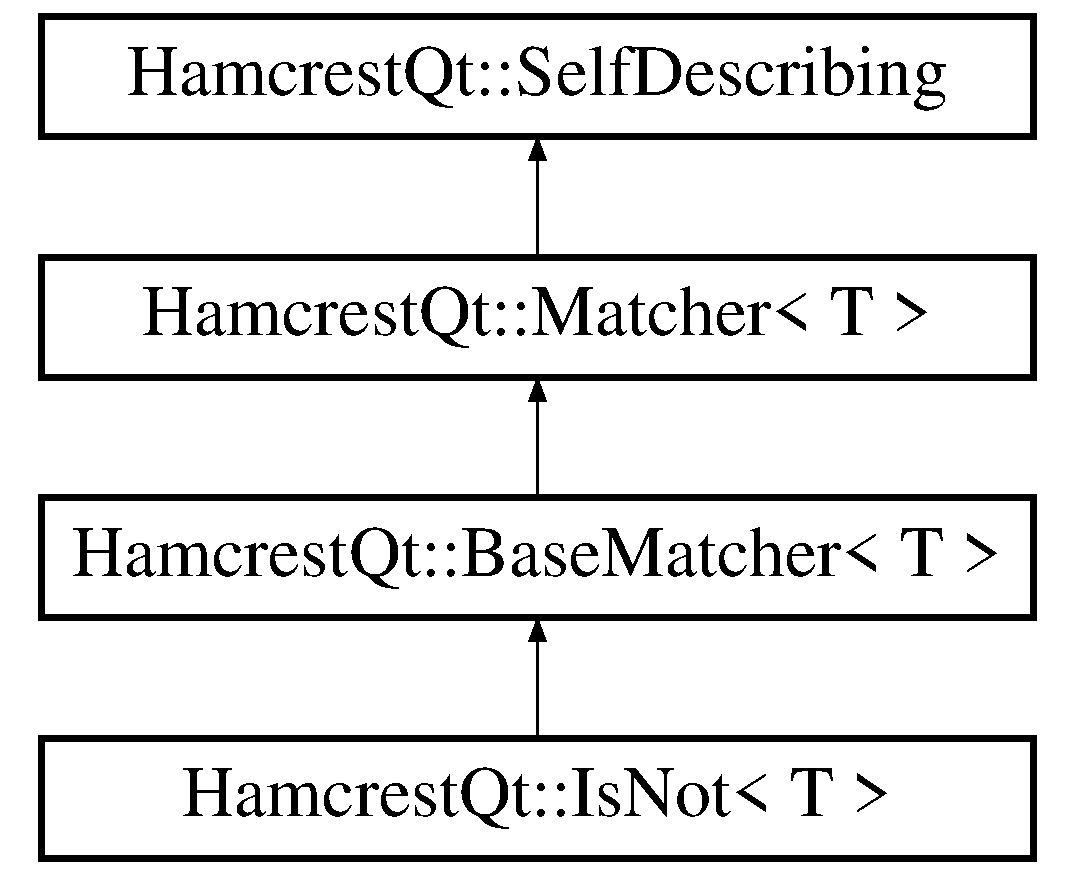
\includegraphics[height=4.000000cm]{class_hamcrest_qt_1_1_is_not}
\end{center}
\end{figure}
\subsection*{Public Member Functions}
\begin{DoxyCompactItemize}
\item 
\hypertarget{class_hamcrest_qt_1_1_is_not_ac31d53bbc1b631f7fa00c5c09568730f}{{\bfseries Is\-Not} (const Q\-Shared\-Pointer$<$ \hyperlink{class_hamcrest_qt_1_1_matcher}{Matcher}$<$ T $>$ $>$ \&m)}\label{class_hamcrest_qt_1_1_is_not_ac31d53bbc1b631f7fa00c5c09568730f}

\item 
virtual bool \hyperlink{class_hamcrest_qt_1_1_is_not_a37c8d69373e96e12dc8937d241cfde9f}{matches} (const T \&item) const 
\begin{DoxyCompactList}\small\item\em Evaluates the matcher for argument {\itshape item}. \end{DoxyCompactList}\item 
virtual void \hyperlink{class_hamcrest_qt_1_1_is_not_a0fe1623440286dcacb586b531e94384f}{describe\-To} (\hyperlink{class_hamcrest_qt_1_1_description}{Description} \&description) const 
\begin{DoxyCompactList}\small\item\em Generates a description of the object. \end{DoxyCompactList}\end{DoxyCompactItemize}


\subsection{Detailed Description}
\subsubsection*{template$<$typename T$>$class Hamcrest\-Qt\-::\-Is\-Not$<$ T $>$}

Calculates the logical negation of a matcher. 

\subsection{Member Function Documentation}
\hypertarget{class_hamcrest_qt_1_1_is_not_a0fe1623440286dcacb586b531e94384f}{\index{Hamcrest\-Qt\-::\-Is\-Not@{Hamcrest\-Qt\-::\-Is\-Not}!describe\-To@{describe\-To}}
\index{describe\-To@{describe\-To}!HamcrestQt::IsNot@{Hamcrest\-Qt\-::\-Is\-Not}}
\subsubsection[{describe\-To}]{\setlength{\rightskip}{0pt plus 5cm}template$<$typename T $>$ virtual void {\bf Hamcrest\-Qt\-::\-Is\-Not}$<$ T $>$\-::describe\-To (
\begin{DoxyParamCaption}
\item[{{\bf Description} \&}]{description}
\end{DoxyParamCaption}
) const\hspace{0.3cm}{\ttfamily [inline]}, {\ttfamily [virtual]}}}\label{class_hamcrest_qt_1_1_is_not_a0fe1623440286dcacb586b531e94384f}


Generates a description of the object. 

The description may be part of a description of a larger object of which this is just a component, so it should be worded appropriately.


\begin{DoxyParams}{Parameters}
{\em description} & The description to be built or appended to. \\
\hline
\end{DoxyParams}


Implements \hyperlink{class_hamcrest_qt_1_1_self_describing_af04da98570148e5e943e42399f718e4c}{Hamcrest\-Qt\-::\-Self\-Describing}.

\hypertarget{class_hamcrest_qt_1_1_is_not_a37c8d69373e96e12dc8937d241cfde9f}{\index{Hamcrest\-Qt\-::\-Is\-Not@{Hamcrest\-Qt\-::\-Is\-Not}!matches@{matches}}
\index{matches@{matches}!HamcrestQt::IsNot@{Hamcrest\-Qt\-::\-Is\-Not}}
\subsubsection[{matches}]{\setlength{\rightskip}{0pt plus 5cm}template$<$typename T $>$ virtual bool {\bf Hamcrest\-Qt\-::\-Is\-Not}$<$ T $>$\-::matches (
\begin{DoxyParamCaption}
\item[{const T \&}]{item}
\end{DoxyParamCaption}
) const\hspace{0.3cm}{\ttfamily [inline]}, {\ttfamily [virtual]}}}\label{class_hamcrest_qt_1_1_is_not_a37c8d69373e96e12dc8937d241cfde9f}


Evaluates the matcher for argument {\itshape item}. 


\begin{DoxyParams}{Parameters}
{\em item} & the object against which the matcher is evaluated. \\
\hline
\end{DoxyParams}
\begin{DoxyReturn}{Returns}
{\ttfamily true} if {\itshape item} matches, otherwise {\ttfamily false}.
\end{DoxyReturn}
\begin{DoxySeeAlso}{See Also}
\hyperlink{class_hamcrest_qt_1_1_base_matcher}{Base\-Matcher} 
\end{DoxySeeAlso}


Implements \hyperlink{class_hamcrest_qt_1_1_matcher_a9a8a775345afd0fde8942a0755303075}{Hamcrest\-Qt\-::\-Matcher$<$ T $>$}.



The documentation for this class was generated from the following file\-:\begin{DoxyCompactItemize}
\item 
C\-:/\-Users/\-Christian/\-Documents/\-Git\-Hub/\-Hamcrest-\/\-Qt/src/core/matcher/isnot.\-h\end{DoxyCompactItemize}

\hypertarget{class_hamcrest_qt_1_1_matcher}{\section{Hamcrest\-Qt\-:\-:Matcher$<$ T $>$ Class Template Reference}
\label{class_hamcrest_qt_1_1_matcher}\index{Hamcrest\-Qt\-::\-Matcher$<$ T $>$@{Hamcrest\-Qt\-::\-Matcher$<$ T $>$}}
}


A matcher over acceptable values.  




{\ttfamily \#include $<$matcher.\-h$>$}

Inheritance diagram for Hamcrest\-Qt\-:\-:Matcher$<$ T $>$\-:\begin{figure}[H]
\begin{center}
\leavevmode
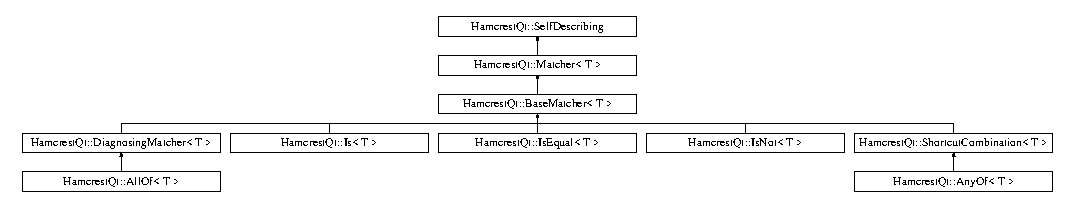
\includegraphics[height=2.343096cm]{class_hamcrest_qt_1_1_matcher}
\end{center}
\end{figure}
\subsection*{Public Member Functions}
\begin{DoxyCompactItemize}
\item 
virtual bool \hyperlink{class_hamcrest_qt_1_1_matcher_a9a8a775345afd0fde8942a0755303075}{matches} (const T \&item) const =0
\begin{DoxyCompactList}\small\item\em Evaluates the matcher for argument {\itshape item}. \end{DoxyCompactList}\item 
virtual void \hyperlink{class_hamcrest_qt_1_1_matcher_aa92292613ca3c83f0501d261de94cb2b}{describe\-Mismatch} (const T \&item, \hyperlink{class_hamcrest_qt_1_1_description}{Description} \&mismatch\-Description) const =0
\begin{DoxyCompactList}\small\item\em Generate a description of why the matcher has not accepted the item. \end{DoxyCompactList}\item 
\hypertarget{class_hamcrest_qt_1_1_matcher_a9b2e61b3e0ffeb3c5fff553c160f70de}{virtual Q\-String {\bfseries to\-String} () const =0}\label{class_hamcrest_qt_1_1_matcher_a9b2e61b3e0ffeb3c5fff553c160f70de}

\end{DoxyCompactItemize}


\subsection{Detailed Description}
\subsubsection*{template$<$typename T$>$class Hamcrest\-Qt\-::\-Matcher$<$ T $>$}

A matcher over acceptable values. 

A matcher is able to describe itself to give feedback when it fails.

\begin{DoxySeeAlso}{See Also}
\hyperlink{class_hamcrest_qt_1_1_base_matcher}{Base\-Matcher} 
\end{DoxySeeAlso}


\subsection{Member Function Documentation}
\hypertarget{class_hamcrest_qt_1_1_matcher_aa92292613ca3c83f0501d261de94cb2b}{\index{Hamcrest\-Qt\-::\-Matcher@{Hamcrest\-Qt\-::\-Matcher}!describe\-Mismatch@{describe\-Mismatch}}
\index{describe\-Mismatch@{describe\-Mismatch}!HamcrestQt::Matcher@{Hamcrest\-Qt\-::\-Matcher}}
\subsubsection[{describe\-Mismatch}]{\setlength{\rightskip}{0pt plus 5cm}template$<$typename T$>$ virtual void {\bf Hamcrest\-Qt\-::\-Matcher}$<$ T $>$\-::describe\-Mismatch (
\begin{DoxyParamCaption}
\item[{const T \&}]{item, }
\item[{{\bf Description} \&}]{mismatch\-Description}
\end{DoxyParamCaption}
) const\hspace{0.3cm}{\ttfamily [pure virtual]}}}\label{class_hamcrest_qt_1_1_matcher_aa92292613ca3c83f0501d261de94cb2b}


Generate a description of why the matcher has not accepted the item. 

The description will be part of a larger description of why a matching failed, so it should be concise. This method assumes that {\ttfamily matches(item)} is false, but will not check this.


\begin{DoxyParams}{Parameters}
{\em item} & The item that the \hyperlink{class_hamcrest_qt_1_1_matcher}{Matcher} has rejected. \\
\hline
{\em mismatch\-Description} & The description to be built or appended to. \\
\hline
\end{DoxyParams}


Implemented in \hyperlink{class_hamcrest_qt_1_1_is_a3a8c6b52b2b0636e24b60542359ba12e}{Hamcrest\-Qt\-::\-Is$<$ T $>$}, \hyperlink{class_hamcrest_qt_1_1_substring_matcher_a23bb6d4b756dd8745a883eb88a993a2b}{Hamcrest\-Qt\-::\-Substring\-Matcher}, \hyperlink{class_hamcrest_qt_1_1_base_matcher_a4299e8a4358ff624fb857a3301dd1b73}{Hamcrest\-Qt\-::\-Base\-Matcher$<$ T $>$}, \hyperlink{class_hamcrest_qt_1_1_base_matcher_a4299e8a4358ff624fb857a3301dd1b73}{Hamcrest\-Qt\-::\-Base\-Matcher$<$ Q\-String $>$}, and \hyperlink{class_hamcrest_qt_1_1_diagnosing_matcher_a122cccc22b8be886b3202e0a126995ed}{Hamcrest\-Qt\-::\-Diagnosing\-Matcher$<$ T $>$}.

\hypertarget{class_hamcrest_qt_1_1_matcher_a9a8a775345afd0fde8942a0755303075}{\index{Hamcrest\-Qt\-::\-Matcher@{Hamcrest\-Qt\-::\-Matcher}!matches@{matches}}
\index{matches@{matches}!HamcrestQt::Matcher@{Hamcrest\-Qt\-::\-Matcher}}
\subsubsection[{matches}]{\setlength{\rightskip}{0pt plus 5cm}template$<$typename T$>$ virtual bool {\bf Hamcrest\-Qt\-::\-Matcher}$<$ T $>$\-::matches (
\begin{DoxyParamCaption}
\item[{const T \&}]{item}
\end{DoxyParamCaption}
) const\hspace{0.3cm}{\ttfamily [pure virtual]}}}\label{class_hamcrest_qt_1_1_matcher_a9a8a775345afd0fde8942a0755303075}


Evaluates the matcher for argument {\itshape item}. 


\begin{DoxyParams}{Parameters}
{\em item} & the object against which the matcher is evaluated. \\
\hline
\end{DoxyParams}
\begin{DoxyReturn}{Returns}
{\ttfamily true} if {\itshape item} matches, otherwise {\ttfamily false}.
\end{DoxyReturn}
\begin{DoxySeeAlso}{See Also}
\hyperlink{class_hamcrest_qt_1_1_base_matcher}{Base\-Matcher} 
\end{DoxySeeAlso}


Implemented in \hyperlink{class_hamcrest_qt_1_1_is_ab8ab441f01e21785134ec0bbfb53f0b4}{Hamcrest\-Qt\-::\-Is$<$ T $>$}, \hyperlink{class_hamcrest_qt_1_1_is_equal_a4a9cc0239c034328baa5aeedf340271f}{Hamcrest\-Qt\-::\-Is\-Equal$<$ T $>$}, \hyperlink{class_hamcrest_qt_1_1_any_of_aa097e760ed6ce642c1ee40c73d73bdce}{Hamcrest\-Qt\-::\-Any\-Of$<$ T $>$}, \hyperlink{class_hamcrest_qt_1_1_is_not_a37c8d69373e96e12dc8937d241cfde9f}{Hamcrest\-Qt\-::\-Is\-Not$<$ T $>$}, \hyperlink{class_hamcrest_qt_1_1_diagnosing_matcher_a95ea76988bacda59586ec1423c4d0e6c}{Hamcrest\-Qt\-::\-Diagnosing\-Matcher$<$ T $>$}, and \hyperlink{class_hamcrest_qt_1_1_substring_matcher_a52111254de729e8ffe6392aaeba1f08b}{Hamcrest\-Qt\-::\-Substring\-Matcher}.



The documentation for this class was generated from the following file\-:\begin{DoxyCompactItemize}
\item 
C\-:/\-Users/\-Christian/\-Documents/\-Git\-Hub/\-Hamcrest-\/\-Qt/src/core/matcher.\-h\end{DoxyCompactItemize}

\hypertarget{class_hamcrest_qt_1_1_matcher_assert}{\section{Hamcrest\-Qt\-:\-:Matcher\-Assert Class Reference}
\label{class_hamcrest_qt_1_1_matcher_assert}\index{Hamcrest\-Qt\-::\-Matcher\-Assert@{Hamcrest\-Qt\-::\-Matcher\-Assert}}
}
\subsection*{Classes}
\begin{DoxyCompactItemize}
\item 
class \hyperlink{class_hamcrest_qt_1_1_matcher_assert_1_1_assertion_listener}{Assertion\-Listener}
\end{DoxyCompactItemize}
\subsection*{Static Public Member Functions}
\begin{DoxyCompactItemize}
\item 
\hypertarget{class_hamcrest_qt_1_1_matcher_assert_aa6ff8e92bdf99e18e23cc52d568f6b35}{static void {\bfseries add\-Assertion\-Listener} (\hyperlink{class_hamcrest_qt_1_1_matcher_assert_1_1_assertion_listener}{Matcher\-Assert\-::\-Assertion\-Listener} $\ast$listener)}\label{class_hamcrest_qt_1_1_matcher_assert_aa6ff8e92bdf99e18e23cc52d568f6b35}

\item 
\hypertarget{class_hamcrest_qt_1_1_matcher_assert_a7ad3b92fda708cc204b3f0e970e220f7}{{\footnotesize template$<$typename T $>$ }\\static bool {\bfseries assert\-That} (const Q\-String \&reason, const T \&actual, const \hyperlink{class_hamcrest_qt_1_1_matcher}{Matcher}$<$ T $>$ \&matcher, const char $\ast$file, int line)}\label{class_hamcrest_qt_1_1_matcher_assert_a7ad3b92fda708cc204b3f0e970e220f7}

\item 
\hypertarget{class_hamcrest_qt_1_1_matcher_assert_aa119900c04bc1e5a86eb39cd73b1ee71}{{\footnotesize template$<$typename T $>$ }\\static bool {\bfseries assert\-That} (const Q\-String \&reason, const T \&actual, const Q\-Shared\-Pointer$<$ \hyperlink{class_hamcrest_qt_1_1_matcher}{Matcher}$<$ T $>$ $>$ \&matcher, const char $\ast$file, int line)}\label{class_hamcrest_qt_1_1_matcher_assert_aa119900c04bc1e5a86eb39cd73b1ee71}

\item 
\hypertarget{class_hamcrest_qt_1_1_matcher_assert_a93a079826e57ef96fb16625d31037572}{{\footnotesize template$<$typename T $>$ }\\static bool {\bfseries assert\-That} (const T \&actual, const \hyperlink{class_hamcrest_qt_1_1_matcher}{Matcher}$<$ T $>$ \&matcher, const char $\ast$file, int line)}\label{class_hamcrest_qt_1_1_matcher_assert_a93a079826e57ef96fb16625d31037572}

\item 
\hypertarget{class_hamcrest_qt_1_1_matcher_assert_a9e72dd2dcc8e0f7ad9f225571b4dbed8}{{\footnotesize template$<$typename T $>$ }\\static bool {\bfseries assert\-That} (const T \&actual, const Q\-Shared\-Pointer$<$ \hyperlink{class_hamcrest_qt_1_1_matcher}{Matcher}$<$ T $>$ $>$ \&matcher, const char $\ast$file, int line)}\label{class_hamcrest_qt_1_1_matcher_assert_a9e72dd2dcc8e0f7ad9f225571b4dbed8}

\item 
\hypertarget{class_hamcrest_qt_1_1_matcher_assert_a29694b80b62cf2d2a71c56ba37398f19}{static bool {\bfseries assert\-That} (const Q\-String \&reason, bool assertion, const char $\ast$file, int line)}\label{class_hamcrest_qt_1_1_matcher_assert_a29694b80b62cf2d2a71c56ba37398f19}

\end{DoxyCompactItemize}


The documentation for this class was generated from the following files\-:\begin{DoxyCompactItemize}
\item 
C\-:/\-Users/\-Christian/\-Documents/\-Git\-Hub/\-Hamcrest-\/\-Qt/src/core/matcherassert.\-h\item 
C\-:/\-Users/\-Christian/\-Documents/\-Git\-Hub/\-Hamcrest-\/\-Qt/src/core/matcherassert.\-cpp\end{DoxyCompactItemize}

\hypertarget{class_hamcrest_qt_1_1_description_1_1_null_description}{\section{Hamcrest\-Qt\-:\-:Description\-:\-:Null\-Description Class Reference}
\label{class_hamcrest_qt_1_1_description_1_1_null_description}\index{Hamcrest\-Qt\-::\-Description\-::\-Null\-Description@{Hamcrest\-Qt\-::\-Description\-::\-Null\-Description}}
}
Inheritance diagram for Hamcrest\-Qt\-:\-:Description\-:\-:Null\-Description\-:\begin{figure}[H]
\begin{center}
\leavevmode
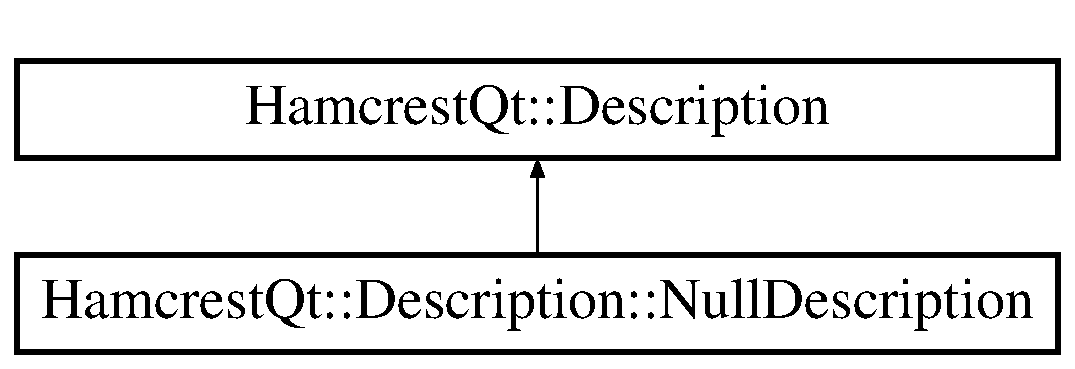
\includegraphics[height=2.000000cm]{class_hamcrest_qt_1_1_description_1_1_null_description}
\end{center}
\end{figure}
\subsection*{Additional Inherited Members}


The documentation for this class was generated from the following file\-:\begin{DoxyCompactItemize}
\item 
C\-:/\-Users/\-Christian/\-Documents/\-Git\-Hub/\-Hamcrest-\/\-Qt/src/core/description.\-cpp\end{DoxyCompactItemize}

\hypertarget{class_hamcrest_qt_1_1_self_describing}{\section{Hamcrest\-Qt\-:\-:Self\-Describing Class Reference}
\label{class_hamcrest_qt_1_1_self_describing}\index{Hamcrest\-Qt\-::\-Self\-Describing@{Hamcrest\-Qt\-::\-Self\-Describing}}
}


The ability of an object to describe itself.  




{\ttfamily \#include $<$selfdescribing.\-h$>$}

Inheritance diagram for Hamcrest\-Qt\-:\-:Self\-Describing\-:\begin{figure}[H]
\begin{center}
\leavevmode
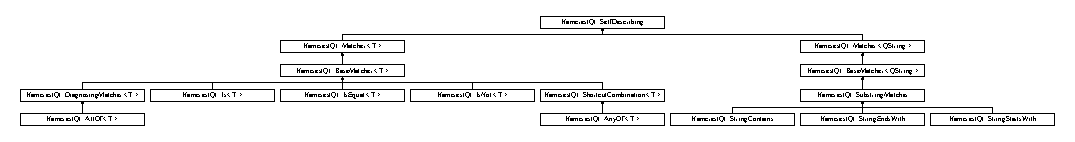
\includegraphics[height=1.464435cm]{class_hamcrest_qt_1_1_self_describing}
\end{center}
\end{figure}
\subsection*{Public Member Functions}
\begin{DoxyCompactItemize}
\item 
virtual void \hyperlink{class_hamcrest_qt_1_1_self_describing_af04da98570148e5e943e42399f718e4c}{describe\-To} (\hyperlink{class_hamcrest_qt_1_1_description}{Description} \&description) const =0
\begin{DoxyCompactList}\small\item\em Generates a description of the object. \end{DoxyCompactList}\end{DoxyCompactItemize}


\subsection{Detailed Description}
The ability of an object to describe itself. 

\subsection{Member Function Documentation}
\hypertarget{class_hamcrest_qt_1_1_self_describing_af04da98570148e5e943e42399f718e4c}{\index{Hamcrest\-Qt\-::\-Self\-Describing@{Hamcrest\-Qt\-::\-Self\-Describing}!describe\-To@{describe\-To}}
\index{describe\-To@{describe\-To}!HamcrestQt::SelfDescribing@{Hamcrest\-Qt\-::\-Self\-Describing}}
\subsubsection[{describe\-To}]{\setlength{\rightskip}{0pt plus 5cm}virtual void Hamcrest\-Qt\-::\-Self\-Describing\-::describe\-To (
\begin{DoxyParamCaption}
\item[{{\bf Description} \&}]{description}
\end{DoxyParamCaption}
) const\hspace{0.3cm}{\ttfamily [pure virtual]}}}\label{class_hamcrest_qt_1_1_self_describing_af04da98570148e5e943e42399f718e4c}


Generates a description of the object. 

The description may be part of a description of a larger object of which this is just a component, so it should be worded appropriately.


\begin{DoxyParams}{Parameters}
{\em description} & The description to be built or appended to. \\
\hline
\end{DoxyParams}


Implemented in \hyperlink{class_hamcrest_qt_1_1_all_of_a0b60757a18e9dc9e9dfd2582cda9d39d}{Hamcrest\-Qt\-::\-All\-Of$<$ T $>$}, \hyperlink{class_hamcrest_qt_1_1_is_adcddba2f01e78feaff9f75ab3c5c7dd2}{Hamcrest\-Qt\-::\-Is$<$ T $>$}, \hyperlink{class_hamcrest_qt_1_1_is_equal_a0f8431cbae42ab84f803c33eb43af260}{Hamcrest\-Qt\-::\-Is\-Equal$<$ T $>$}, \hyperlink{class_hamcrest_qt_1_1_any_of_a32a386c0a8f6bab40344199964c3d62f}{Hamcrest\-Qt\-::\-Any\-Of$<$ T $>$}, \hyperlink{class_hamcrest_qt_1_1_is_not_a0fe1623440286dcacb586b531e94384f}{Hamcrest\-Qt\-::\-Is\-Not$<$ T $>$}, and \hyperlink{class_hamcrest_qt_1_1_substring_matcher_af3f68e4871350cdecdf145575593e671}{Hamcrest\-Qt\-::\-Substring\-Matcher}.



The documentation for this class was generated from the following file\-:\begin{DoxyCompactItemize}
\item 
C\-:/\-Users/\-Christian/\-Documents/\-Git\-Hub/\-Hamcrest-\/\-Qt/src/core/selfdescribing.\-h\end{DoxyCompactItemize}

\hypertarget{class_hamcrest_qt_1_1_shortcut_combination}{\section{Hamcrest\-Qt\-:\-:Shortcut\-Combination$<$ T $>$ Class Template Reference}
\label{class_hamcrest_qt_1_1_shortcut_combination}\index{Hamcrest\-Qt\-::\-Shortcut\-Combination$<$ T $>$@{Hamcrest\-Qt\-::\-Shortcut\-Combination$<$ T $>$}}
}
Inheritance diagram for Hamcrest\-Qt\-:\-:Shortcut\-Combination$<$ T $>$\-:\begin{figure}[H]
\begin{center}
\leavevmode
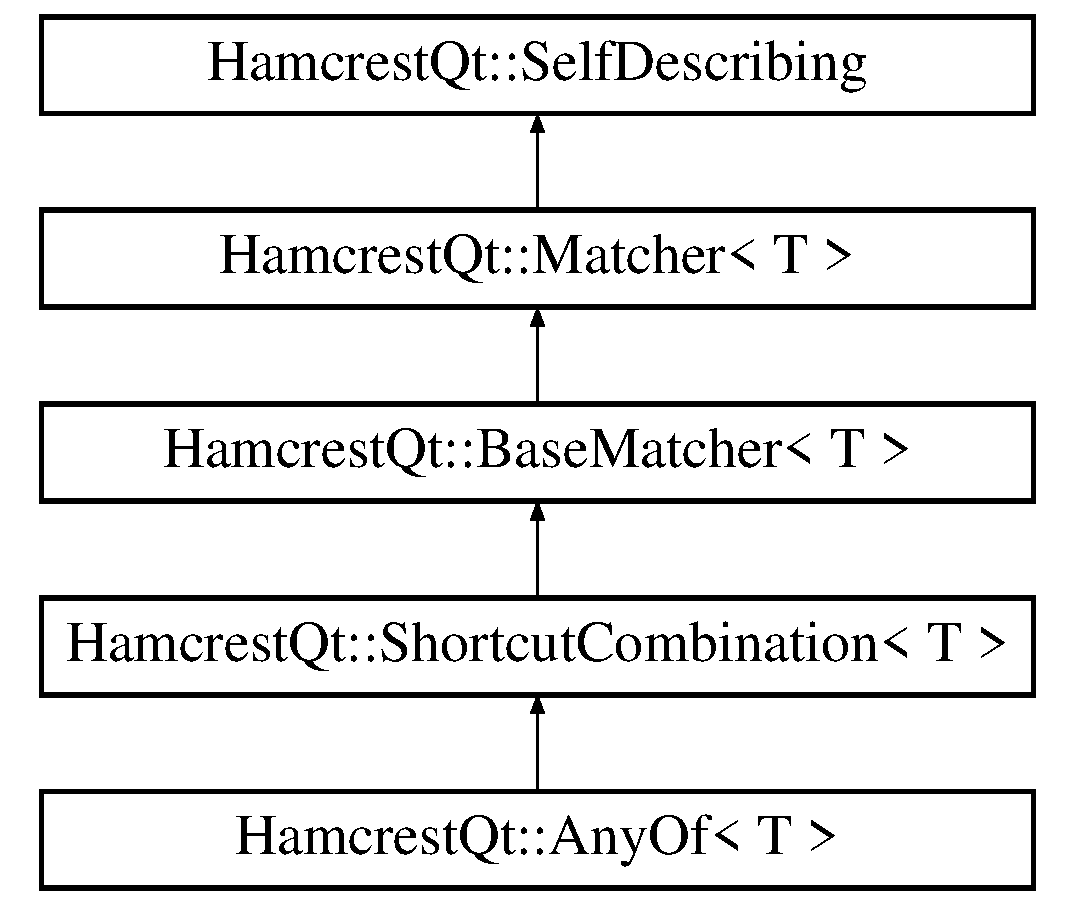
\includegraphics[height=5.000000cm]{class_hamcrest_qt_1_1_shortcut_combination}
\end{center}
\end{figure}
\subsection*{Public Member Functions}
\begin{DoxyCompactItemize}
\item 
\hypertarget{class_hamcrest_qt_1_1_shortcut_combination_a5a9786df3928fbfb67c5f49c8fc3f520}{{\bfseries Shortcut\-Combination} (const Q\-List$<$ Q\-Shared\-Pointer$<$ \hyperlink{class_hamcrest_qt_1_1_matcher}{Matcher}$<$ T $>$ $>$ $>$ \&m)}\label{class_hamcrest_qt_1_1_shortcut_combination_a5a9786df3928fbfb67c5f49c8fc3f520}

\item 
\hypertarget{class_hamcrest_qt_1_1_shortcut_combination_ad00ac5caacd1944e0e9e8bf6e38aa8cf}{void {\bfseries describe\-To} (\hyperlink{class_hamcrest_qt_1_1_description}{Description} \&description, const Q\-String \&op) const }\label{class_hamcrest_qt_1_1_shortcut_combination_ad00ac5caacd1944e0e9e8bf6e38aa8cf}

\end{DoxyCompactItemize}
\subsection*{Protected Member Functions}
\begin{DoxyCompactItemize}
\item 
\hypertarget{class_hamcrest_qt_1_1_shortcut_combination_a74bee98c726131fcb588633d54581a9e}{virtual bool {\bfseries matches} (const T \&item, bool shortcut) const }\label{class_hamcrest_qt_1_1_shortcut_combination_a74bee98c726131fcb588633d54581a9e}

\end{DoxyCompactItemize}


The documentation for this class was generated from the following file\-:\begin{DoxyCompactItemize}
\item 
C\-:/\-Users/\-Christian/\-Documents/\-Git\-Hub/\-Hamcrest-\/\-Qt/src/core/matcher/shortcutcombination.\-h\end{DoxyCompactItemize}

\hypertarget{class_hamcrest_qt_1_1_string_contains}{\section{Hamcrest\-Qt\-:\-:String\-Contains Class Reference}
\label{class_hamcrest_qt_1_1_string_contains}\index{Hamcrest\-Qt\-::\-String\-Contains@{Hamcrest\-Qt\-::\-String\-Contains}}
}


Tests if the argument is a string that contains a substring.  




{\ttfamily \#include $<$stringcontains.\-h$>$}

Inheritance diagram for Hamcrest\-Qt\-:\-:String\-Contains\-:\begin{figure}[H]
\begin{center}
\leavevmode
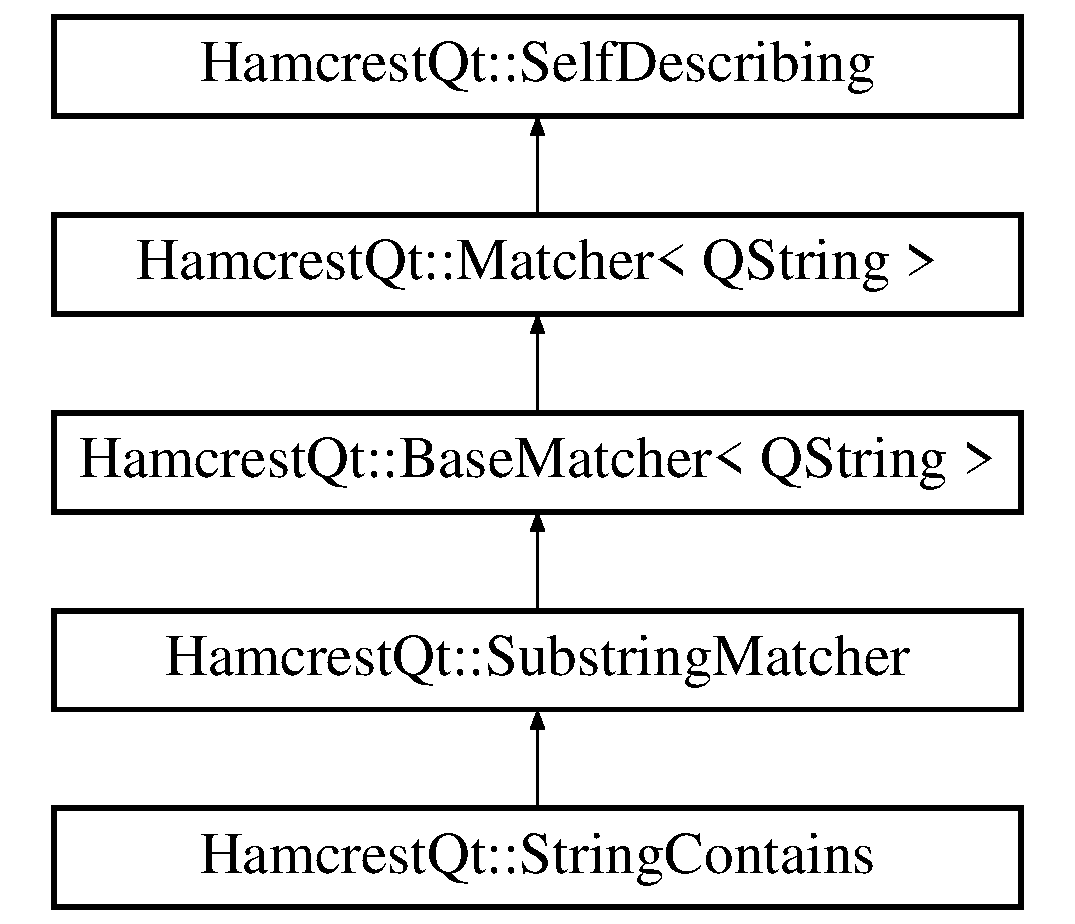
\includegraphics[height=5.000000cm]{class_hamcrest_qt_1_1_string_contains}
\end{center}
\end{figure}
\subsection*{Public Member Functions}
\begin{DoxyCompactItemize}
\item 
\hypertarget{class_hamcrest_qt_1_1_string_contains_a95fb26986696b078679b543c7cebf778}{{\bfseries String\-Contains} (const Q\-String \&substring)}\label{class_hamcrest_qt_1_1_string_contains_a95fb26986696b078679b543c7cebf778}

\end{DoxyCompactItemize}
\subsection*{Protected Member Functions}
\begin{DoxyCompactItemize}
\item 
\hypertarget{class_hamcrest_qt_1_1_string_contains_ae799a4bc7a53fa9bb2cbcd9ed516710b}{virtual bool {\bfseries eval\-Substring\-Of} (const Q\-String \&str) const }\label{class_hamcrest_qt_1_1_string_contains_ae799a4bc7a53fa9bb2cbcd9ed516710b}

\item 
\hypertarget{class_hamcrest_qt_1_1_string_contains_a69c4bb24421ea1c010d9d053315218fa}{virtual Q\-String {\bfseries relationship} () const }\label{class_hamcrest_qt_1_1_string_contains_a69c4bb24421ea1c010d9d053315218fa}

\end{DoxyCompactItemize}
\subsection*{Additional Inherited Members}


\subsection{Detailed Description}
Tests if the argument is a string that contains a substring. 

The documentation for this class was generated from the following files\-:\begin{DoxyCompactItemize}
\item 
C\-:/\-Users/\-Christian/\-Documents/\-Git\-Hub/\-Hamcrest-\/\-Qt/src/core/matcher/stringcontains.\-h\item 
C\-:/\-Users/\-Christian/\-Documents/\-Git\-Hub/\-Hamcrest-\/\-Qt/src/core/matcher/stringcontains.\-cpp\end{DoxyCompactItemize}

\hypertarget{class_hamcrest_qt_1_1_string_description}{\section{Hamcrest\-Qt\-:\-:String\-Description Class Reference}
\label{class_hamcrest_qt_1_1_string_description}\index{Hamcrest\-Qt\-::\-String\-Description@{Hamcrest\-Qt\-::\-String\-Description}}
}


A \hyperlink{class_hamcrest_qt_1_1_description}{Description} that is stored as a string.  




{\ttfamily \#include $<$stringdescription.\-h$>$}

Inheritance diagram for Hamcrest\-Qt\-:\-:String\-Description\-:\begin{figure}[H]
\begin{center}
\leavevmode
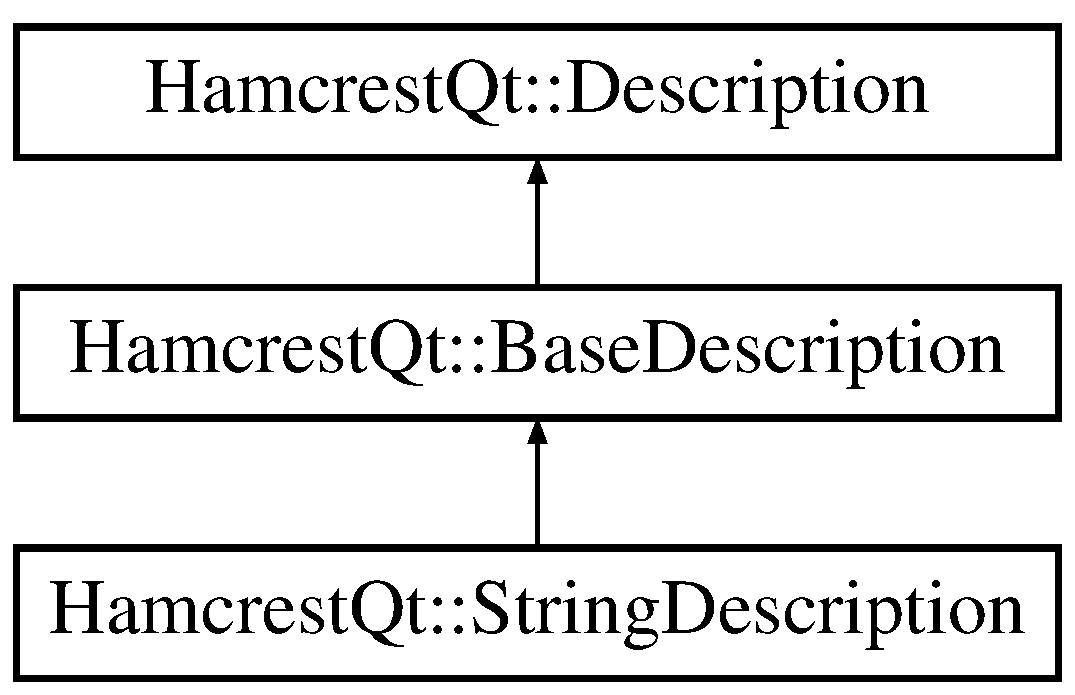
\includegraphics[height=3.000000cm]{class_hamcrest_qt_1_1_string_description}
\end{center}
\end{figure}
\subsection*{Public Member Functions}
\begin{DoxyCompactItemize}
\item 
\hypertarget{class_hamcrest_qt_1_1_string_description_a7e5471e0482e2c026af2d37e5c155e67}{virtual Q\-String \hyperlink{class_hamcrest_qt_1_1_string_description_a7e5471e0482e2c026af2d37e5c155e67}{to\-String} () const }\label{class_hamcrest_qt_1_1_string_description_a7e5471e0482e2c026af2d37e5c155e67}

\begin{DoxyCompactList}\small\item\em Returns the description as a string. \end{DoxyCompactList}\end{DoxyCompactItemize}
\subsection*{Static Public Member Functions}
\begin{DoxyCompactItemize}
\item 
static Q\-String \hyperlink{class_hamcrest_qt_1_1_string_description_aa7cffb8dd9c5502076dd58554395b906}{to\-String} (const \hyperlink{class_hamcrest_qt_1_1_self_describing}{Self\-Describing} \&self\-Describing)
\begin{DoxyCompactList}\small\item\em Return the description of a \hyperlink{class_hamcrest_qt_1_1_self_describing}{Self\-Describing} object as a {\ttfamily Q\-String}. \end{DoxyCompactList}\item 
\hypertarget{class_hamcrest_qt_1_1_string_description_a426e3c8524d7e72075aa3e8b974b5bc8}{static Q\-String \hyperlink{class_hamcrest_qt_1_1_string_description_a426e3c8524d7e72075aa3e8b974b5bc8}{as\-String} (const \hyperlink{class_hamcrest_qt_1_1_self_describing}{Self\-Describing} \&self\-Describing)}\label{class_hamcrest_qt_1_1_string_description_a426e3c8524d7e72075aa3e8b974b5bc8}

\begin{DoxyCompactList}\small\item\em Alias for \hyperlink{}{to\-String(\-Self\-Describing)}. \end{DoxyCompactList}\end{DoxyCompactItemize}
\subsection*{Protected Member Functions}
\begin{DoxyCompactItemize}
\item 
virtual void \hyperlink{class_hamcrest_qt_1_1_string_description_a2e27da55b34506521df58b3e2f22a48c}{append\-String} (const Q\-String \&str)
\begin{DoxyCompactList}\small\item\em Append the String {\itshape str} to the description. \end{DoxyCompactList}\item 
\hypertarget{class_hamcrest_qt_1_1_string_description_ad259aeffbdd7d6d51cd636ed98b3bd38}{virtual void {\bfseries append} (const Q\-Char \&c)}\label{class_hamcrest_qt_1_1_string_description_ad259aeffbdd7d6d51cd636ed98b3bd38}

\end{DoxyCompactItemize}


\subsection{Detailed Description}
A \hyperlink{class_hamcrest_qt_1_1_description}{Description} that is stored as a string. 

\subsection{Member Function Documentation}
\hypertarget{class_hamcrest_qt_1_1_string_description_a2e27da55b34506521df58b3e2f22a48c}{\index{Hamcrest\-Qt\-::\-String\-Description@{Hamcrest\-Qt\-::\-String\-Description}!append\-String@{append\-String}}
\index{append\-String@{append\-String}!HamcrestQt::StringDescription@{Hamcrest\-Qt\-::\-String\-Description}}
\subsubsection[{append\-String}]{\setlength{\rightskip}{0pt plus 5cm}void Hamcrest\-Qt\-::\-String\-Description\-::append\-String (
\begin{DoxyParamCaption}
\item[{const Q\-String \&}]{str}
\end{DoxyParamCaption}
)\hspace{0.3cm}{\ttfamily [protected]}, {\ttfamily [virtual]}}}\label{class_hamcrest_qt_1_1_string_description_a2e27da55b34506521df58b3e2f22a48c}


Append the String {\itshape str} to the description. 

The default implementation passes every character to \hyperlink{}{append(\-Q\-Char)}. Override in subclasses to provide an efficient implementation. 

Reimplemented from \hyperlink{class_hamcrest_qt_1_1_base_description_a7bb209dee8a47c3b4346a8126d0f0b3c}{Hamcrest\-Qt\-::\-Base\-Description}.

\hypertarget{class_hamcrest_qt_1_1_string_description_aa7cffb8dd9c5502076dd58554395b906}{\index{Hamcrest\-Qt\-::\-String\-Description@{Hamcrest\-Qt\-::\-String\-Description}!to\-String@{to\-String}}
\index{to\-String@{to\-String}!HamcrestQt::StringDescription@{Hamcrest\-Qt\-::\-String\-Description}}
\subsubsection[{to\-String}]{\setlength{\rightskip}{0pt plus 5cm}Q\-String Hamcrest\-Qt\-::\-String\-Description\-::to\-String (
\begin{DoxyParamCaption}
\item[{const {\bf Self\-Describing} \&}]{self\-Describing}
\end{DoxyParamCaption}
)\hspace{0.3cm}{\ttfamily [static]}}}\label{class_hamcrest_qt_1_1_string_description_aa7cffb8dd9c5502076dd58554395b906}


Return the description of a \hyperlink{class_hamcrest_qt_1_1_self_describing}{Self\-Describing} object as a {\ttfamily Q\-String}. 


\begin{DoxyParams}{Parameters}
{\em self\-Describing} & The object to be described. \\
\hline
\end{DoxyParams}
\begin{DoxyReturn}{Returns}
The description of the object. 
\end{DoxyReturn}


The documentation for this class was generated from the following files\-:\begin{DoxyCompactItemize}
\item 
C\-:/\-Users/\-Christian/\-Documents/\-Git\-Hub/\-Hamcrest-\/\-Qt/src/core/stringdescription.\-h\item 
C\-:/\-Users/\-Christian/\-Documents/\-Git\-Hub/\-Hamcrest-\/\-Qt/src/core/stringdescription.\-cpp\end{DoxyCompactItemize}

\hypertarget{class_hamcrest_qt_1_1_string_ends_with}{\section{Hamcrest\-Qt\-:\-:String\-Ends\-With Class Reference}
\label{class_hamcrest_qt_1_1_string_ends_with}\index{Hamcrest\-Qt\-::\-String\-Ends\-With@{Hamcrest\-Qt\-::\-String\-Ends\-With}}
}


Tests if the argument is a string that ends with a substring.  




{\ttfamily \#include $<$stringendswith.\-h$>$}

Inheritance diagram for Hamcrest\-Qt\-:\-:String\-Ends\-With\-:\begin{figure}[H]
\begin{center}
\leavevmode
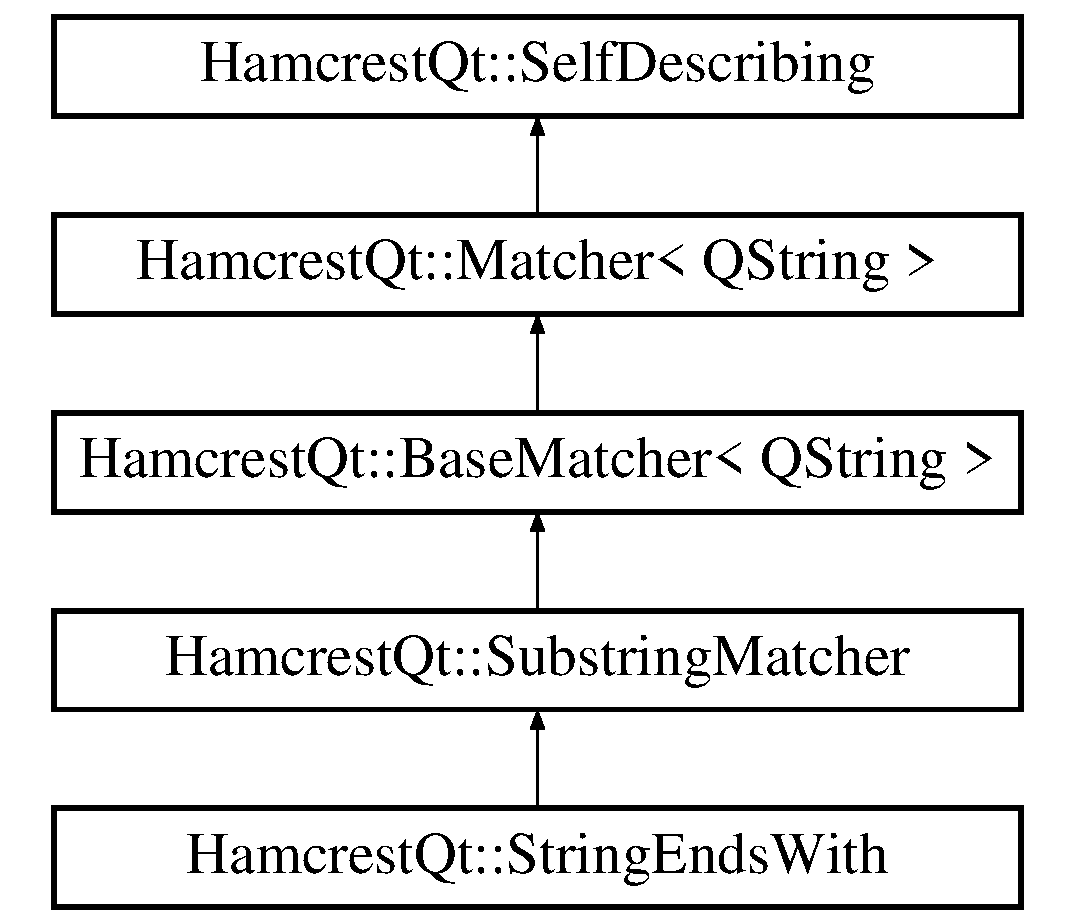
\includegraphics[height=5.000000cm]{class_hamcrest_qt_1_1_string_ends_with}
\end{center}
\end{figure}
\subsection*{Public Member Functions}
\begin{DoxyCompactItemize}
\item 
\hypertarget{class_hamcrest_qt_1_1_string_ends_with_af01e4ae95d7664b021cc646c0330c5a4}{{\bfseries String\-Ends\-With} (const Q\-String \&substring)}\label{class_hamcrest_qt_1_1_string_ends_with_af01e4ae95d7664b021cc646c0330c5a4}

\end{DoxyCompactItemize}
\subsection*{Protected Member Functions}
\begin{DoxyCompactItemize}
\item 
\hypertarget{class_hamcrest_qt_1_1_string_ends_with_a897370fa94bf442b9626e7bcddee1973}{virtual bool {\bfseries eval\-Substring\-Of} (const Q\-String \&str) const }\label{class_hamcrest_qt_1_1_string_ends_with_a897370fa94bf442b9626e7bcddee1973}

\item 
\hypertarget{class_hamcrest_qt_1_1_string_ends_with_a4a77869c52f296be516f7f1165f2d9cc}{virtual Q\-String {\bfseries relationship} () const }\label{class_hamcrest_qt_1_1_string_ends_with_a4a77869c52f296be516f7f1165f2d9cc}

\end{DoxyCompactItemize}
\subsection*{Additional Inherited Members}


\subsection{Detailed Description}
Tests if the argument is a string that ends with a substring. 

The documentation for this class was generated from the following files\-:\begin{DoxyCompactItemize}
\item 
C\-:/\-Users/\-Christian/\-Documents/\-Git\-Hub/\-Hamcrest-\/\-Qt/src/core/matcher/stringendswith.\-h\item 
C\-:/\-Users/\-Christian/\-Documents/\-Git\-Hub/\-Hamcrest-\/\-Qt/src/core/matcher/stringendswith.\-cpp\end{DoxyCompactItemize}

\hypertarget{class_hamcrest_qt_1_1_string_starts_with}{\section{Hamcrest\-Qt\-:\-:String\-Starts\-With Class Reference}
\label{class_hamcrest_qt_1_1_string_starts_with}\index{Hamcrest\-Qt\-::\-String\-Starts\-With@{Hamcrest\-Qt\-::\-String\-Starts\-With}}
}


Tests if the argument is a string that starts with a substring.  




{\ttfamily \#include $<$stringstartswith.\-h$>$}

Inheritance diagram for Hamcrest\-Qt\-:\-:String\-Starts\-With\-:\begin{figure}[H]
\begin{center}
\leavevmode
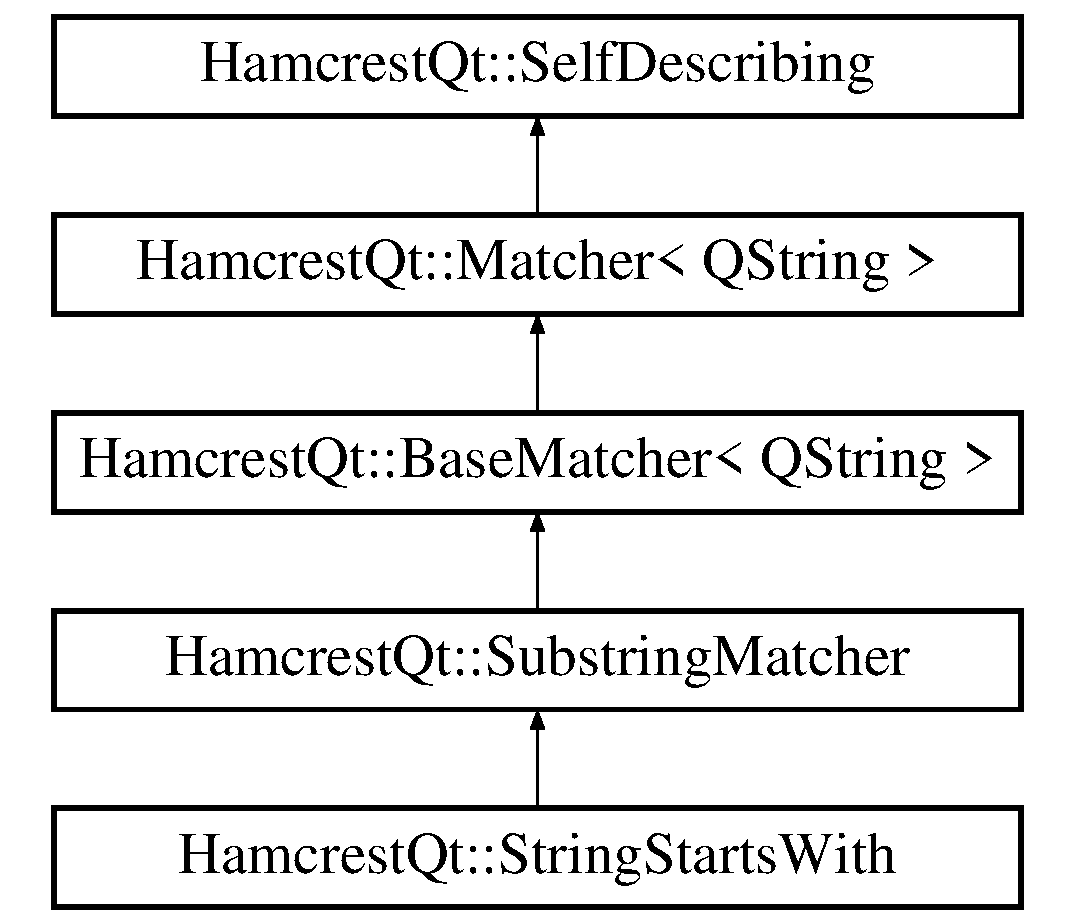
\includegraphics[height=5.000000cm]{class_hamcrest_qt_1_1_string_starts_with}
\end{center}
\end{figure}
\subsection*{Public Member Functions}
\begin{DoxyCompactItemize}
\item 
\hypertarget{class_hamcrest_qt_1_1_string_starts_with_a5b7e2876a5eba8a0217668d9557ad207}{{\bfseries String\-Starts\-With} (const Q\-String \&substring)}\label{class_hamcrest_qt_1_1_string_starts_with_a5b7e2876a5eba8a0217668d9557ad207}

\end{DoxyCompactItemize}
\subsection*{Protected Member Functions}
\begin{DoxyCompactItemize}
\item 
\hypertarget{class_hamcrest_qt_1_1_string_starts_with_a828dbdcea8bb9910c178bd65473f9451}{virtual bool {\bfseries eval\-Substring\-Of} (const Q\-String \&str) const }\label{class_hamcrest_qt_1_1_string_starts_with_a828dbdcea8bb9910c178bd65473f9451}

\item 
\hypertarget{class_hamcrest_qt_1_1_string_starts_with_ad06efdaa236c839403a7843779924e02}{virtual Q\-String {\bfseries relationship} () const }\label{class_hamcrest_qt_1_1_string_starts_with_ad06efdaa236c839403a7843779924e02}

\end{DoxyCompactItemize}
\subsection*{Additional Inherited Members}


\subsection{Detailed Description}
Tests if the argument is a string that starts with a substring. 

The documentation for this class was generated from the following files\-:\begin{DoxyCompactItemize}
\item 
C\-:/\-Users/\-Christian/\-Documents/\-Git\-Hub/\-Hamcrest-\/\-Qt/src/core/matcher/stringstartswith.\-h\item 
C\-:/\-Users/\-Christian/\-Documents/\-Git\-Hub/\-Hamcrest-\/\-Qt/src/core/matcher/stringstartswith.\-cpp\end{DoxyCompactItemize}

\hypertarget{class_hamcrest_qt_1_1_substring_matcher}{\section{Hamcrest\-Qt\-:\-:Substring\-Matcher Class Reference}
\label{class_hamcrest_qt_1_1_substring_matcher}\index{Hamcrest\-Qt\-::\-Substring\-Matcher@{Hamcrest\-Qt\-::\-Substring\-Matcher}}
}
Inheritance diagram for Hamcrest\-Qt\-:\-:Substring\-Matcher\-:\begin{figure}[H]
\begin{center}
\leavevmode
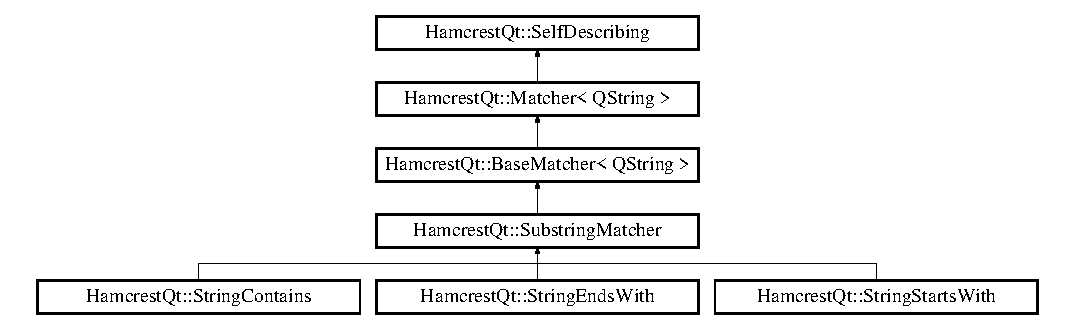
\includegraphics[height=3.988604cm]{class_hamcrest_qt_1_1_substring_matcher}
\end{center}
\end{figure}
\subsection*{Public Member Functions}
\begin{DoxyCompactItemize}
\item 
virtual bool \hyperlink{class_hamcrest_qt_1_1_substring_matcher_a52111254de729e8ffe6392aaeba1f08b}{matches} (const Q\-String \&item) const 
\begin{DoxyCompactList}\small\item\em Evaluates the matcher for argument {\itshape item}. \end{DoxyCompactList}\item 
virtual void \hyperlink{class_hamcrest_qt_1_1_substring_matcher_af3f68e4871350cdecdf145575593e671}{describe\-To} (\hyperlink{class_hamcrest_qt_1_1_description}{Description} \&description) const 
\begin{DoxyCompactList}\small\item\em Generates a description of the object. \end{DoxyCompactList}\item 
virtual void \hyperlink{class_hamcrest_qt_1_1_substring_matcher_a23bb6d4b756dd8745a883eb88a993a2b}{describe\-Mismatch} (const Q\-String \&item, \hyperlink{class_hamcrest_qt_1_1_description}{Description} \&description) const 
\begin{DoxyCompactList}\small\item\em Generate a description of why the matcher has not accepted the item. \end{DoxyCompactList}\end{DoxyCompactItemize}
\subsection*{Protected Member Functions}
\begin{DoxyCompactItemize}
\item 
\hypertarget{class_hamcrest_qt_1_1_substring_matcher_a8a4045b70e21e0faf4942f3933aa1d35}{{\bfseries Substring\-Matcher} (const Q\-String \&str)}\label{class_hamcrest_qt_1_1_substring_matcher_a8a4045b70e21e0faf4942f3933aa1d35}

\item 
\hypertarget{class_hamcrest_qt_1_1_substring_matcher_ac8b42a97691518d7f2332b7fb1c930d6}{virtual bool {\bfseries eval\-Substring\-Of} (const Q\-String \&str) const =0}\label{class_hamcrest_qt_1_1_substring_matcher_ac8b42a97691518d7f2332b7fb1c930d6}

\item 
\hypertarget{class_hamcrest_qt_1_1_substring_matcher_a86c109697dbaaf2b012dc774f9fa9668}{virtual Q\-String {\bfseries relationship} () const =0}\label{class_hamcrest_qt_1_1_substring_matcher_a86c109697dbaaf2b012dc774f9fa9668}

\end{DoxyCompactItemize}
\subsection*{Protected Attributes}
\begin{DoxyCompactItemize}
\item 
\hypertarget{class_hamcrest_qt_1_1_substring_matcher_acea1b88931a3a8ae858ae18ba9aa5911}{Q\-String {\bfseries substring}}\label{class_hamcrest_qt_1_1_substring_matcher_acea1b88931a3a8ae858ae18ba9aa5911}

\end{DoxyCompactItemize}


\subsection{Member Function Documentation}
\hypertarget{class_hamcrest_qt_1_1_substring_matcher_a23bb6d4b756dd8745a883eb88a993a2b}{\index{Hamcrest\-Qt\-::\-Substring\-Matcher@{Hamcrest\-Qt\-::\-Substring\-Matcher}!describe\-Mismatch@{describe\-Mismatch}}
\index{describe\-Mismatch@{describe\-Mismatch}!HamcrestQt::SubstringMatcher@{Hamcrest\-Qt\-::\-Substring\-Matcher}}
\subsubsection[{describe\-Mismatch}]{\setlength{\rightskip}{0pt plus 5cm}virtual void Hamcrest\-Qt\-::\-Substring\-Matcher\-::describe\-Mismatch (
\begin{DoxyParamCaption}
\item[{const Q\-String \&}]{item, }
\item[{{\bf Description} \&}]{mismatch\-Description}
\end{DoxyParamCaption}
) const\hspace{0.3cm}{\ttfamily [inline]}, {\ttfamily [virtual]}}}\label{class_hamcrest_qt_1_1_substring_matcher_a23bb6d4b756dd8745a883eb88a993a2b}


Generate a description of why the matcher has not accepted the item. 

The description will be part of a larger description of why a matching failed, so it should be concise. This method assumes that {\ttfamily matches(item)} is false, but will not check this.


\begin{DoxyParams}{Parameters}
{\em item} & The item that the \hyperlink{class_hamcrest_qt_1_1_matcher}{Matcher} has rejected. \\
\hline
{\em mismatch\-Description} & The description to be built or appended to. \\
\hline
\end{DoxyParams}


Reimplemented from \hyperlink{class_hamcrest_qt_1_1_base_matcher_a4299e8a4358ff624fb857a3301dd1b73}{Hamcrest\-Qt\-::\-Base\-Matcher$<$ Q\-String $>$}.

\hypertarget{class_hamcrest_qt_1_1_substring_matcher_af3f68e4871350cdecdf145575593e671}{\index{Hamcrest\-Qt\-::\-Substring\-Matcher@{Hamcrest\-Qt\-::\-Substring\-Matcher}!describe\-To@{describe\-To}}
\index{describe\-To@{describe\-To}!HamcrestQt::SubstringMatcher@{Hamcrest\-Qt\-::\-Substring\-Matcher}}
\subsubsection[{describe\-To}]{\setlength{\rightskip}{0pt plus 5cm}virtual void Hamcrest\-Qt\-::\-Substring\-Matcher\-::describe\-To (
\begin{DoxyParamCaption}
\item[{{\bf Description} \&}]{description}
\end{DoxyParamCaption}
) const\hspace{0.3cm}{\ttfamily [inline]}, {\ttfamily [virtual]}}}\label{class_hamcrest_qt_1_1_substring_matcher_af3f68e4871350cdecdf145575593e671}


Generates a description of the object. 

The description may be part of a description of a larger object of which this is just a component, so it should be worded appropriately.


\begin{DoxyParams}{Parameters}
{\em description} & The description to be built or appended to. \\
\hline
\end{DoxyParams}


Implements \hyperlink{class_hamcrest_qt_1_1_self_describing_af04da98570148e5e943e42399f718e4c}{Hamcrest\-Qt\-::\-Self\-Describing}.

\hypertarget{class_hamcrest_qt_1_1_substring_matcher_a52111254de729e8ffe6392aaeba1f08b}{\index{Hamcrest\-Qt\-::\-Substring\-Matcher@{Hamcrest\-Qt\-::\-Substring\-Matcher}!matches@{matches}}
\index{matches@{matches}!HamcrestQt::SubstringMatcher@{Hamcrest\-Qt\-::\-Substring\-Matcher}}
\subsubsection[{matches}]{\setlength{\rightskip}{0pt plus 5cm}virtual bool Hamcrest\-Qt\-::\-Substring\-Matcher\-::matches (
\begin{DoxyParamCaption}
\item[{const Q\-String \&}]{item}
\end{DoxyParamCaption}
) const\hspace{0.3cm}{\ttfamily [inline]}, {\ttfamily [virtual]}}}\label{class_hamcrest_qt_1_1_substring_matcher_a52111254de729e8ffe6392aaeba1f08b}


Evaluates the matcher for argument {\itshape item}. 


\begin{DoxyParams}{Parameters}
{\em item} & the object against which the matcher is evaluated. \\
\hline
\end{DoxyParams}
\begin{DoxyReturn}{Returns}
{\ttfamily true} if {\itshape item} matches, otherwise {\ttfamily false}.
\end{DoxyReturn}
\begin{DoxySeeAlso}{See Also}
\hyperlink{class_hamcrest_qt_1_1_base_matcher}{Base\-Matcher} 
\end{DoxySeeAlso}


Implements \hyperlink{class_hamcrest_qt_1_1_matcher_a9a8a775345afd0fde8942a0755303075}{Hamcrest\-Qt\-::\-Matcher$<$ Q\-String $>$}.



The documentation for this class was generated from the following file\-:\begin{DoxyCompactItemize}
\item 
C\-:/\-Users/\-Christian/\-Documents/\-Git\-Hub/\-Hamcrest-\/\-Qt/src/core/matcher/substringmatcher.\-h\end{DoxyCompactItemize}

%--- End generated contents ---

% Index
\newpage
\phantomsection
\addcontentsline{toc}{part}{Index}
\printindex

\end{document}
